\cotefile{144}
\scanpage{1}
\figure{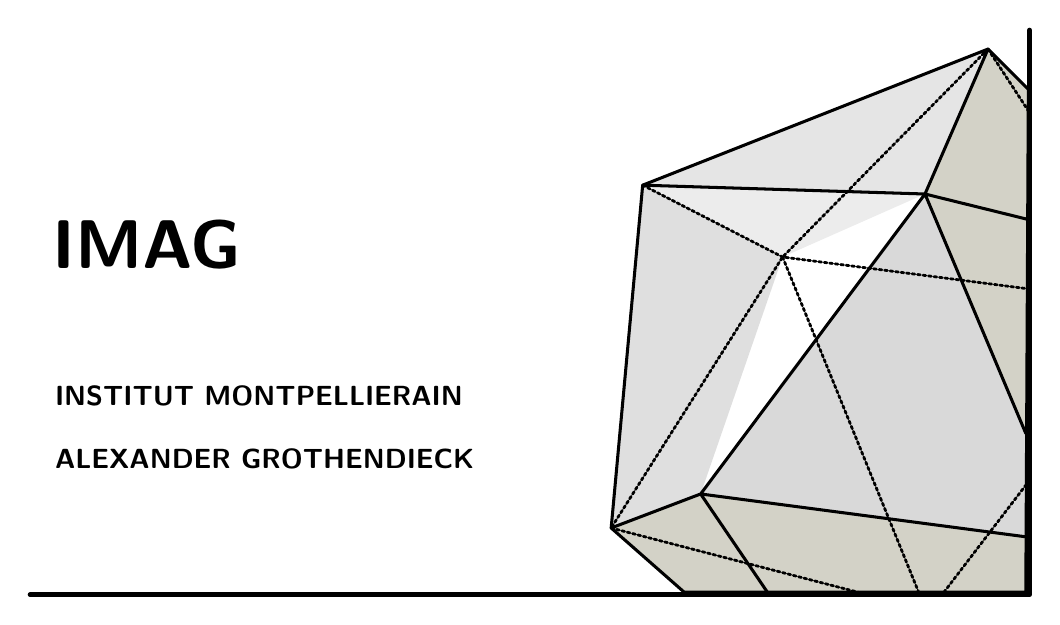
\begin{tikzpicture}[x=0.016cm,y=0.016cm,line cap=round,line join=round]
\node[anchor=west,font=\sffamily\bfseries\Huge] at (20,300) {IMAG};
\node[anchor=west,font=\sffamily\bfseries] at (22,180) {INSTITUT MONTPELLIERAIN};
\node[anchor=west,font=\sffamily\bfseries] at (22,130) {ALEXANDER GROTHENDIECK};
\fill[gray!20] (496,347)--(770,455)--(720,340)--cycle;
\fill[gray!15] (496,347)--(720,340)--(607,290)--cycle;
\fill[gray!25] (496,347)--(607,290)--(542,102)--(471,75)--cycle;
\fill[gray!30] (542,102)--(720,340)--(800,150)--(800,68)--cycle;
\fill[yellow!12!gray!45] (720,340)--(770,455)--(802,423)--(801,320)--cycle;
\fill[yellow!12!gray!45] (720,340)--(801,320)--(800,150)--cycle;
\fill[yellow!12!gray!45] (471,75)--(542,102)--(800,68)--(800,24)--(529,24)--cycle;
\draw[line width=1.1pt] (471,75)--(496,347)--(770,455)--(802,423)--(800,24)--(529,24)--cycle;
\draw[line width=1.1pt] (496,347)--(720,340)--(801,320) (770,455)--(720,340)--(800,150) (720,340)--(542,102)--(471,75) (542,102)--(595,24) (542,102)--(800,68);
\draw[densely dotted,line width=1pt] (496,347)--(607,290)--(800,265) (770,455)--(607,290)--(471,75) (607,290)--(715,24) (770,455)--(802,406) (471,75)--(667,24) (735,24)--(800,109);
\draw[line width=1.8pt] (10,22)--(803,22)--(803,470);
\end{tikzpicture}}

\scanpage{2}
Discussion avec

Deligne

+ \unsure{lettr.} Barry Mazur

\mspage{1}

\scanpage{3}
Conversations avec Deligne du 30.5 et 5.6.
\margin{\unsure{i}}

1) Pour groupes finis opérant sur surfaces : utiliser ``th de Smith'' (contre \unsure{patholog}) pour prouver que \unsure{les} ens des points fixes \unsure{est une} variété homologique du pt de vue local -- donc si \unsure{dim 1} loc. connexe, donc connexe par arcs...

2) Exemple de Bing d'une involution de $B^3$ ayant un \unsure{ens} de pts fixes sauvage (\inserted{\unsure{genre}} sphère d'Alexander) mais dont la restriction à $S^2=\partial B^3$ est la conj. complexe.

3) Il doit y avoir des actions \inserted{\unsure{différentiables}} de groupes finis sur $B^n$ ($n\geq\deleted{\unsure{3\ 4}}\ 5$ ?) qui ne sont pas le cône d'une action sur $S^{n-1}=\partial B^n$. Lié au fait qu'une action \deleted{\unsure{linéaire} \illegible{1}} d'un groupe fini sur une sphère \deleted{\unsure{ce disque} \illegible{3}} \inserted{avec pt fixe} n'est pas \unsure{néc\textsuperscript{t}} contenue dans un conjugué \inserted{topologique} du groupe orthogonal. (J'ai pas bien compris comment...)

4) Nécessité de faire intervenir la forme \unsure{intersect.} (à valeurs dans $\unsure{T}$) pour décrire \deleted{la \unsure{forme}} structure ``arithmétique'' du groupe fondamental d'une courbe lisse propre connexe sur $k$ \unsure{alg.} clos. Question de définir algébriquement les intersections de ``chemins'' (au sens théorie des revêtements)

\figure{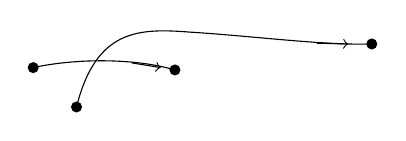
\begin{tikzpicture}[x=1cm,y=1cm]
\fill (0,0) circle (2pt) (1.8,-.03) circle (2pt) (.55,-.5) circle (2pt) (4.3,.3) circle (2pt);
\draw (0,0) .. controls (.55,.12) and (1.3,.12) .. (1.8,-.03);
\draw[->] (1.25,.06)--(1.62,0);
\draw (.55,-.5) .. controls (.8,.5) and (1.35,.5) .. (2,.45) .. controls (2.8,.4) and (3.7,.28) .. (4.3,.3);
\draw[->] (3.6,.31)--(4,.3);
\end{tikzpicture}}

Donner théorie cohomologique d'une courbe dans le \unsure{prodisque|prodiscret}

......

\figure{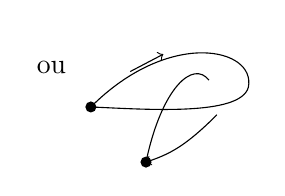
\begin{tikzpicture}[x=1cm,y=1cm]
\node at (-.5,.5) {ou};
\fill (0,0) circle (2pt) (.7,-.7) circle (2pt);
\draw (0,0) .. controls (1,1) and (2.1,.75) .. (2,.25) .. controls (1.9,-.12) and (.7,-.03) .. (0,0);
\draw[->] (.5,.45)--(.92,.67);
\draw (.7,-.7) .. controls (.9,.25) and (1.3,.6) .. (1.5,.34);
\draw[->] (1.6,-.1) .. controls (1.2,-.5) and (1,-.6) .. (.7,-.7);
\end{tikzpicture}}
\figure{\begin{tikzpicture}[x=1cm,y=1cm]
\node at (-.8,1.2) {ou};
\fill (0,.5) circle (2pt) (.9,.9) circle (2pt) (1.1,-.7) circle (2pt);
\draw (0,.5) .. controls (1.3,2) and (1.6,1.4) .. (1.15,.65) .. controls (.8,.3) and (.3,.45) .. (0,.5);
\draw[->] (.72,.45)--(.35,.45);
\draw[->] (.9,.9) .. controls (.83,.1) and (1,-.35) .. (1.1,-.7);
\end{tikzpicture}}

\mspage{2}

\scanpage{4}
5) Compactification des types modulaires $M_{g,\nu}$ et structure à l'infini. Il semble qu'on ait
\[
\pi_1(\widehat M_{g,\nu})=1\qquad\text{si }g\geq2
\]
(si $g=1$, $\nu=0$, le $\pi_1$ doit être cyclique fini d'ordre pair divisant 12...), et $\pi_1(M_{g,\nu}^{\infty})=1$ itou.

$*$ Déf. de $\widehat M_{g,\nu}$ : schémas \inserted{$X/S$} propres (\unsure{projectifs} ?) \inserted{$X/S$ muni d'\unsure{sections} $(f_1,-f_\nu)$,} et plats sur $S$, de prés. finie, à fibres $X_s$ géom connexes réduites, n'ayant que des pts doubles ordinaires, et les $f_{is}$ étant des pts lisses, enfin le groupe des autom. de $(X_s,f_{1s},\ldots,f_{\nu s})$ étant fini (ce qui signifie que \deleted{\unsure{les}} composante irréductible de genre $0$ de $X_s$ a au moins trois points marqués -- soit par intersection avec d'autres comp. irréd, soit comme pts $f_{is}$ ...)

$*$ Question : si $\nu=0$, $X_s^{\inserted{\text{lisse}}}$ est-il contenu dans sa jacobienne, \unsure{\`a} extension d'une VA par un tore ?

$*$ La vérification du critère valuatif semble étrange.

Les générateurs ``twist'' de $\unsure{\Gamma}_{g\nu}$ sont les lacets autour des comp. irréductibles de $M_{g,\nu}^{\infty}$

\mspage{3}

\scanpage{5}
6) Nécessité, en dim $>1$, d'une description plus délicate de la ``structure à l'infini'' d'un schéma lisse connexe \inserted{\unsure{séparé !}} sur $k$ alg. clos.

$X$
\diagram{\begin{tikzcd}[column sep=large]
1\arrow[r]&\pi_1^\infty(X)\arrow[r,"i"]&\pi_1(X)\arrow[r]&\pi_1(\widehat X)\arrow[r]&1\\
1\arrow[r]&\pi_1^\infty(U)\arrow[r]\arrow[u,"\alpha"]&\pi_1(U)\arrow[r]\arrow[u]&\pi_1(\mathfrak X)\arrow[r]\arrow[u]\arrow[d,equal]&1\\
&&&\pi_1(Y)&
\end{tikzcd}}
\inserted{\unsure{compactifié}}

\deleted{$\unsure{U\subset\widehat X\supset Y}$}
\diagram{\begin{tikzcd}
U\arrow[r,phantom,"\subset"]\arrow[d]&\mathfrak X\arrow[d]&\text{complété formel de}\;\widehat X\;\text{le long de }Y\\
X\arrow[r,phantom,"\subset"]&\widehat X\arrow[r,phantom,"\supset"]&Y(=\widehat X\setminus X)
\end{tikzcd}}

$\pi_1^\infty(X)$ est le sous-groupe \deleted{\unsure{clos}} \inserted{fermé} de $\pi_1(X)$ engendré par $\alpha(\pi_1^\infty(U))$, mais $\alpha$ n'est pas néc. surjectif.

Il faudrait expliciter, \inserted{en car. $0$ disons,} en termes de
\[
\Pi=\varprojlim\unsure{\pi_1}(U)
\]
et de la structure \inserted{``combinatoire''} de $Y$ (qu'on peut supposer diviseur à croisements normaux) le gpe $\pi_1^\infty(U)$ et l'action de Galois dessus, et exiger que \inserted{l'hom. ext.} $i\circ\alpha:\pi_1^\infty(U)\longrightarrow\pi_1(X)$ commute à l'action de Galois...

On doit pouvoir \inserted{par Lefschetz} faire une réduction au cas $\dim X=2$ ....

7) Sur l'espace de Teichmüller \inserted{complexe} $\widetilde M_{g,\nu\deleted{\unsure{\mathbb C}}}^{\unsure{an}}=\unsure{\mathcal M}_{g,\nu}^{\unsure{an}}$ (rev. universel de \unsure{la multiplicité} \inserted{\unsure{anal.}} $M_{g\nu}^{\unsure{an}}\unsure{(\mathbb C)}$)

\mspage{4}

\scanpage{6}
on n'a pas défini pour l'instant de métrique riemannienne intrinsèque intéressante, mais bien des métriques finslériennes. On espère trouver une métrique riemannienne à \uline{courbure négative}, qui permettrait alors par un argument géométrique simple (en utilisant \inserted{l'existence et} l'unicité de la géodésique qui joint deux pts) de prouver que tt gpe fini d'autom. complexes de $\mathcal M_{g,\nu}$ admet un pt fixe. Deligne pense que c'est vrai que tt sous gpe fini de $\Gamma_{g,\nu}$ a un pt fixe dans $\mathcal M_{g,\nu}$, et il ne voit que cette voie d'approche plausible.

\figure{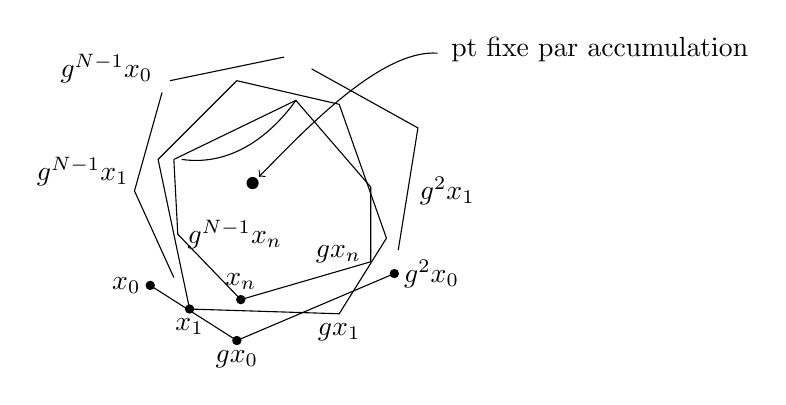
\begin{tikzpicture}[x=1cm,y=1cm]
\draw (-1.6,-.8)--(-.5,-1.5)--(1.5,-.65);
\draw (-1.3,-.7)--(-1.8,.4)--(-1.45,1.65);
\draw (-1.35,1.8)--(.1,2.1);
\draw (.45,1.95)--(1.8,1.2)--(1.55,-.35);
\draw (-1.1,-1.1)--(.8,-1.16)--(1.4,-.2)--(.8,1.5)--(-.5,1.8)--(-1.5,.8)--(-1.1,-1.1);
\draw (-1.3,.8)--(.25,1.55)--(1.2,.45)--(1.2,-.5)--(-.45,-.98)--(-1.25,-.15)--(-1.3,.8);
\draw (-1.2,.8)..controls (-.5,.7) and (0,1.2)..(.25,1.55);
\fill (-1.6,-.8) circle(1.7pt) (-1.1,-1.1) circle(1.7pt) (-.5,-1.5) circle(1.7pt) (1.5,-.65) circle(1.7pt) (-.45,-.98) circle(1.7pt) (-.3,.5) circle(2.2pt);
\node[left] at (-1.6,-.8) {$x_0$};\node[below] at (-1.1,-1.1) {$x_1$};
\node[below] at (-.5,-1.5) {$gx_0$};\node[below] at (.8,-1.16) {$gx_1$};
\node[right] at (1.5,-.65) {$g^2x_0$};\node[right] at (1.7,.4) {$g^2x_1$};
\node[left] at (-1.45,1.95) {$g^{\unsure{N-1}}x_0$};
\node[left] at (-1.75,.65) {$g^{\unsure{N-1}}x_1$};
\node[above] at (-.45,-.98) {$x_n$};\node[left] at (1.2,-.4) {$gx_n$};
\node[right] at (-1.25,-.15) {$g^{\unsure{N-1}}x_n$};
\node[right] at (2.1,2.2) {pt fixe par accumulation};
\draw[->] (2.05,2.15)..controls (1.3,2.2) and (.3,1.1)..(-.22,.58);
\end{tikzpicture}}

8) Mumford connaîtrait la présentation des $\Gamma_{g,\nu}$ (via les générateurs habituels).

L. Bers (Columbia.) ferait de la ``chirurgie complexe'' des surfaces de Riemann pour \deleted{\unsure{définir}} étudier la compactification des $M_{g,\nu}$.

\mspage{5}

\scanpage{7}
9) Le cône sur une variété compacte $S$ peut être une variété à bord, sans que $S$ soit une sphère.

Exemple : considérons le ss-groupe $\Gamma\subset S^3$ d'ordre $120$, \deleted{\unsure{image réciproque}} de $\underset{\substack{\Vert\\ A}}{\unsure{\mathfrak S}_5^+}\subset\underbrace{S^3/\mathord{\pm}1}_{SO(3,\mathbb R)}$. Considérons
\[
S^3/\Gamma\simeq SO(3,\mathbb R)/A\simeq\text{variété des icosaèdres}
\]
\inserted{réguliers} inscrits dans une sphère donnée. Ce n'est pas une sphère, ni sa suspension, qui n'est pas une variété (elle a deux pts singuliers, en lesquels le groupe fondamental local est $\simeq\Gamma$, donc non trivial) Mais \deleted{elle} \inserted{c'est un} \inserted{espace} simplement connexe $S$. \deleted{Sa suspension} \deleted{est encore} Le produit par une droite est néanmoins une variété (?), et sa suspension est une variété \inserted{et $\simeq S^5$,} -- y compris aux deux ``pôles'' ....

\margin{Edwards\par \uline{Exposé Bourbaki}\par 1977 ou 78\par (\unsure{Latour|Lalonde}, 515)}
\margin{$X$ variété de dim $n$, $\mathbb Z$-\unsure{sphère} homologique, sa double susp. est une sphère}

Pour donner des conditions \deleted{topologiques} \inserted{de lissité de nature $\neq$ topolog.} sur un espace à stratification \unsure{str\textsuperscript{t}} conique, \deleted{\unsure{qui impliqueraient que}} \inserted{qui \unsure{viseraient à} \deleted{\illegible{2}}} faire que certains espaces soient des sphères \deleted{topologiques}, il faudrait d'après Deligne se placer dans un cadre

\mspage{6}

\scanpage{8}
tel que le PL (ou d'autres meilleurs, à la \unsure{Hironaka} p.ex.), le cadre topologique pur ne s'y prêtant pas. Il semble néanmoins que dans le cas des \unsure{n-cartes|cartes} loc. finies \uline{régulières}, les difficultés disparaissent \deleted{\unsure{topologiques}}
\margin{à vérifier avec soin ....}

10) Les gpes apparaissant comme groupes d'automorphismes de ``cartes régulières \deleted{\unsure{(du pt de v\textsuperscript{u})}} \uline{simplement connexes} (loc finies ?), \deleted{\unsure{orientées}} \inserted{\unsure{orientées}} ou pas, sont tous des groupes de Coxeter. Ceux parmi eux qui sont finis sont bien connus (cf livre Bourbaki) -- il semble qu'ils correspondent tous à des sphères -- avec la décomposition cellulaire ``simpliciale'' évidente, liée à la géométrie des gpes de Coxeter.
\margin{id}

D'après Deligne, toutes les ``cartes régulières (finies ou non) \inserted{simplement connexes} devraient

\mspage{7}

\scanpage{9}
figurer dans Bourbaki (pavages coniques, affines etc) -- tout au moins dans le cas \deleted{\unsure{alg}} non singulier. \inserted{Dans le cas infini,} les cas sembleraient liés (identiques ?) à celui où la forme quadratique invariante est (au signe près) de signature $(1,\unsure{--1})$ -- ce qui signifie que la sphère unité se décompose en deux composantes connexes \uline{simplement connexes} : c'est une de ces composantes qui est \inserted{doit} être le siège de la \deleted{\unsure{de la}} carte, on prend les traces dessus des cônes simpliciaux déduits (par op. de $G$) de l'un d'eux...

11) Lien entre l'icosaèdre et $E_8$ : la \deleted{\unsure{f}} forme quadratique de degré $4$ sur
\[
\mathbb Z[\alpha]=\mathbb Z[T]/(T^2+T-1)=\text{anneau des}
\]
entiers de $\mathbb Q(\tfrac12(-1\pm\sqrt5))=\mathbb Q(\sqrt5)$, composée avec la trace, donne la forme quadratique de $E_8$ .... d'où syst. de racines de $E_8$ .... Mais Attention : la ramification
\margin{?}

\mspage{8}

\scanpage{10}
Dear Shurik,

I have been asking people about the questions you raised in your letter. Each day I postpone writing to you, thinking that I could send more complete answers the next day. But since it is getting close to the time \deleted{that you} when \deleted{you arrive} you will be coming to visit, I'll send off these rather incomplete comments. The end of May , beginning of June seem to be fine for me, Deligne. As for me I must lecture on mondays, but \deleted{\unsure{most of}} other days are free. Do you want a room at Ormaille?

The answer to Question (a) seems to be no. Here is a sketch of an example that Deligne made up. Let $H$ be the group generated by $x,y$ with the relations $x^3=y^3=1$, and $xyx^{-1}y^{-1}$ is central. Let $C$ be the (infinite cyclic) group generated by $xyx^{-1}y^{-1}$. So:
\diagram{\begin{tikzcd}
1\arrow[r]&C\arrow[r]&H\arrow[r]&\Gamma\arrow[r]&1
\end{tikzcd}}
(where $\Gamma=\mathbb Z/3\mathbb Z\times\mathbb Z/3\mathbb Z$).

Now let $G$ be the universal cover of $SL_2\ \mathbb R$, and identify the infinite cyclic group $C$ with the center of $G$. By a (noncommutative group analogue of) pushout, Deligne constructs an extension
\diagram{\begin{tikzcd}
1\arrow[r]&C\arrow[r]\arrow[d]&H\arrow[r]\arrow[d,dashed]&\Gamma\arrow[r]\arrow[d,"="]&1\\
1\arrow[r]&G\arrow[r,dashed]&E\arrow[r]&\Gamma\arrow[r]&0
\end{tikzcd}}
which doesn't split.

The answer to (b) seems to be yes for Lie groups, but beyond that I don't know. E.g. whether a contractible group \inserted{(\unsure{$\infty$-dim'l})} can have elements of finite order.

The question about the cone is answered negatively. Namely, there is an involution of $B^3$ with a circle fixed point set in the boundary $S^2$ (indeed a tame circle) yet whose fixed point set in the interior is wild. \inserted{(a Bing-type example)}

The question about finite subgroups of the Teichmuller group seems to be related to recent work of Thurston, but I don't yet know the full story there.

\margin{\deleted{\unsure{Barry}} (t.s.v.p)}
\figure{\begin{tikzpicture}[x=1cm,y=1cm]\draw[->] (1,.8)..controls (1.2,.5) and (.5,.25)..(0,0);\end{tikzpicture}}

Best, et à bientôt

Barry

\mspage{9}

\scanpage{11}
\mspage{10}

I just checked with Siebenmann and a Teichmuller space expert named \unsure{Haritz} -- The situation is this:

\textcircled{1} It is unknown whether every finite subgroup $\Gamma\subseteq$ Teich. group operates on an algebraic curve. But

\textcircled{2} It is true for $\Gamma=$ finite soluble gp +

\textcircled{3} True \deleted{\unsure{also}} for genus $=2$.

\figure{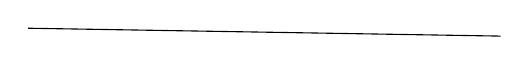
\begin{tikzpicture}\draw (0,0)--(6,-.1);\end{tikzpicture}}

Concerning the hypersurface $Y\subseteq X$ and finite autom. $u$ of $X$ which is \uline{identity} on $\unsure{X|Y}$ -- Siebenmann says that this is certainly solvable using \uline{Smith Theory} (i.e. $u=1$).

\scanpage{13}
\mspage{\textcircled{1}}
\margin{1982}
\diagram{\begin{tikzcd}[column sep=large]
\mathcal X_{g,\nu\mathbb Q}\simeq M_{g,\nu+1,\nu\mathbb Q}\arrow[r,no head]\arrow[d,no head]&\mathcal X_{g,\nu\mathbb C}\simeq M_{g,\nu+1,\nu\mathbb C}\arrow[r,no head]\arrow[d,no head]&\mathcal X_{g,\nu}^{an}\simeq M_{g,\nu+1,\nu}^{an}\arrow[d,no head]\\
M_{g,\nu\mathbb Q}\arrow[r,no head]\arrow[d,no head]&M_{g,\nu\mathbb C}\arrow[r,no head]\arrow[d,no head]&M_{g,\nu}^{an}\\
\mathbb Q\arrow[r,no head]&\mathbb C&
\end{tikzcd}}

\[
\left\{\begin{array}{l}
X_{g,\nu}\ \text{courbe alg/}\mathbb C\quad\text{type }g,\nu,\ \text{corr. à}\quad
\xi_0\in\operatorname{Ob}\uline{\mathrm{Pt}}(M_{g,\nu\mathbb Q};\mathbb C)\simeq\operatorname{Ob}\uline{\mathrm{Pt}}(M_{g,\nu\mathbb C}/\mathbb C)\\
\phantom{X_{g,\nu}}\simeq(\mathcal X_{g,\nu})_{\xi_0}\hfill\simeq\operatorname{Ob}\uline{\mathrm{Pt}}(M_{g,\nu}^{an})
\end{array}\right.
\]
\[
x_0\in X_{g,\nu}(\mathbb C)\simeq X_{g,\nu}^{an},\quad (X_0,x_0)\ \text{corr. :}\quad
\xi_0\in\operatorname{Ob}\uline{\mathrm{Pt}}(\mathcal X_{g,\nu\mathbb Q};\mathbb C)\simeq\operatorname{Ob}\uline{\mathrm{Pt}}(\mathcal X_{g,\nu\mathbb C}/\mathbb C)
\deleted{\unsure{\simeq}}\simeq\operatorname{Ob}\uline{\mathrm{Pt}}(\mathcal X_{g,\nu}^{an})
\]
au dessus de $\xi_0$

\uline{Déf}
\[
(1)\quad\left\{\begin{array}{l}
\Gamma_{g,\nu}^{+}=\pi_1(M_{g,\nu}^{an},\xi_0)\\
\mathcal G_{g,\nu}^{+}=\pi_1(\mathcal X_{g,\nu}^{an},x_0)\simeq\Gamma_{g,\nu+1,\nu}\subset\Gamma_{g,\nu+1}\\
\Pi_{g,\nu}=\pi_1(X_{g,\nu},x_0)\\[4pt]
\mathcal N_{g,\nu}=\pi_1(M_{g,\nu\mathbb Q},\xi_0)\\
\mathcal M_{g,\nu}=\pi_1(\mathcal X_{g,\nu\mathbb Q},x_0)
\end{array}\right.
\]
\deleted{\illegible{1}}

d'où
\diagram{\begin{tikzcd}[column sep=small]
(2)\quad1\arrow[r]&\Pi_{g,\nu}\arrow[r]\arrow[d,equal]&\mathcal G^+_{g,\nu}\arrow[r]\arrow[d,hook]&\Gamma^+_{g,\nu}\arrow[r]\arrow[d,hook]&1\\
1\arrow[r]&\Pi_{g,\nu}\arrow[r]&\operatorname{Aut}_{loc}(\Pi_{g,\nu})\arrow[r]&\operatorname{Autext}_{loc}(\Pi_{g,\nu})&
\end{tikzcd}}

\deleted{et} et, en passant aux complétés \deleted{et}
\diagram{\begin{tikzcd}[column sep=small]
(3)\quad1\arrow[r]&\widehat\Pi_{g,\nu}\arrow[r]\arrow[d,equal]&\widehat{\mathcal G}^+_{g,\nu}\arrow[r]\arrow[d,hook,"?"']&\widehat\Gamma^+_{g,\nu}\arrow[r]\arrow[d,hook,"?"]&1\\
1\arrow[r]&\widehat\Pi_{g,\nu}\arrow[r]&\operatorname{Aut}_{loc}(\widehat\Pi_{g,\nu})\arrow[r]&\operatorname{Autext}_{loc}\unsure{(}&
\end{tikzcd}}

\deleted{$\widehat\Pi_{g,\nu}\overset{can}{\simeq}\pi_1(X_{g,\nu\mathbb C},x_0)$}
\[
(4)\quad\left\{\begin{array}{l}
\widehat\Gamma^+_{g,\nu}\overset{can}{\simeq}\pi_1(M_{g,\nu\mathbb C},\xi_0)\overset{can}{\simeq}\pi_1(M_{g,\nu\overline{\mathbb Q}},\xi_0)\\
\widehat{\mathcal G}^+_{g,\nu}\overset{can}{\simeq}\pi_1(\deleted{M}\mathcal X_{g,\nu\mathbb C},x_0)\overset{can}{\simeq}\pi_1(\mathcal X_{g,\nu\overline{\mathbb Q}},x_0)\simeq\widehat\Gamma_{g,\nu+1,\nu}\subset\widehat\Gamma_{g,\nu+1}\\
\widehat\Pi_{g,\nu}\overset{can}{\simeq}\pi_1(X_{g,\nu\mathbb C},x_0)\simeq\pi_1(X_{g,\nu\overline{\mathbb Q}},x_0)
\end{array}\right.
\]
\deleted{$\unsure{\widehat\Pi_{g,\nu}}$}

\diagram{\begin{tikzcd}[column sep=large]
&1&1&&\\
1\arrow[r]&\widehat\Gamma^+_{g,\nu}\arrow[r]\arrow[u]&\mathcal N_{g,\nu}\arrow[r,no head]\arrow[u]&\Gamma_{\overline{\mathbb Q}/\mathbb Q}\arrow[r,no head]&1\\
(5)\quad1\arrow[r,no head]&\widehat{\mathcal G}^+_{g,\nu}\arrow[r]\arrow[u]&\mathcal M_{g,\nu}\arrow[r,no head]\arrow[u]&\Gamma_{\overline{\mathbb Q}/\mathbb Q}\arrow[r,no head]\arrow[u,equal]&1\\
&\widehat\Pi_{g,\nu}\arrow[r,Rightarrow]\arrow[u]&\widehat\Pi_{g,\nu}\arrow[u]&&\\
&1\arrow[u]&1\arrow[u]&&
\end{tikzcd}}
\[\underbrace{\hspace{5em}}_{(3)}\]

\margin{\deleted{$\unsure{(6)\ 1\to\widehat\Pi_{g,\nu}\to\mathcal M_{g,\nu}\to\mathcal N_{g,\nu}\to1}$}}
\margin{\uline{NB} $\widehat\Gamma_{g,\nu},\widehat{\mathcal G}_{g,\nu}$ s'obtiennent comme images inverses de $\{1,\tau\}\subset\Gamma_{\overline{\mathbb Q}/\mathbb Q}$ ($\tau\in\Gamma_{\overline{\mathbb Q}/\mathbb Q}$, conj. complexe) dans $\mathcal N_{g,\nu},\mathcal M_{g,\nu}$}

\uline{NB} On a (via $\mathcal N_{g,\nu}\to\operatorname{Autext}_{loc}\widehat\Pi_{g,\nu}$ p.ex.)
\diagram{\begin{tikzcd}
\Gamma^+_{g,\nu}\arrow[r]&\widehat\Gamma^+_{g,\nu}\arrow[r]&\mathcal N_{g,\nu}\arrow[r,Rightarrow]&\boxed{\mathfrak S_\nu}\\
(\unsure{7})\quad\mathcal G_{g,\nu}\arrow[r,no head]\arrow[u]&\widehat{\mathcal G}_{g,\nu}\arrow[r,no head]\arrow[u]&\mathcal M_{g,\nu}\arrow[u]&
\end{tikzcd}}

d'où, en prenant les noyaux, des groupes
\[
(8)\quad\left\{\begin{array}{l}
\Gamma^{+!}_{g,\nu},\ \widehat\Gamma^{+!}_{g,\nu},\ \mathcal N^!_{g,\nu}\\
\mathcal G^{+!}_{g,\nu},\ \widehat{\mathcal G}^{+!}_{g,\nu},\ \mathcal M^!_{g,\nu}
\end{array}\right.
\]
s'interprétant comme des $\pi_1$ également ...

\mspage{12}
Il y a des des suites ``en $!$''
\deleted{\unsure{TSVP}} $(2')\ (3')\ (5')$

\figure{
\begin{tikzpicture}\draw (0,0) ellipse (.65 and .25);\node at (0,0) {TSVP!};\end{tikzpicture}}

\scanpage{14}
\diagram{\begin{tikzcd}[column sep=small]
(9)\quad1\arrow[r,no head]&\widehat\Pi_{g,\nu}\arrow[r,no head]\arrow[d,"1"]&\mathcal M_{g,\nu}\arrow[r,no head]\arrow[d,hook,"?"']&\mathcal N_{g,\nu}\arrow[r]\arrow[d,hook,"?"']&1\\
1\arrow[r,no head]&\widehat\Pi_{g,\nu}\arrow[r]&\unsure{\operatorname{Autl}|\operatorname{Aut}}_{loc}(\widehat\Pi_{g,\nu})\arrow[r]&\operatorname{Autext}_{loc}(\widehat\Pi_{g,\nu})\arrow[r,no head]&1
\end{tikzcd}}

prolongeant (2) et (3). On a donc que l'image $\unsure{\mathcal M'|\mathcal N'}_{g,\nu}$ de $\unsure{\mathcal M|\mathcal N}_{g,\nu}$ dans $\operatorname{Aut}^{\unsure{*}}_{loc}(\unsure{\overline\Pi|\widehat\Pi}_{g,\nu})$ normalise celle $\widehat\Gamma'_{g,\nu}$ de $\widehat\Gamma^+_{g,\nu}$ (la partie ``Teichmüller profini'') et l'on a
\[
(10)\qquad \mathcal M'_{g,\nu}/\Gamma'_{g,\nu}\simeq\text{quotient de }\Gamma_{\overline{\mathbb Q}/\mathbb Q}
\]

\uline{NB} on peut prouver que pour $g$ fixé, $\nu$ grand, c'est un isom. avec $\Gamma_{\overline{\mathbb Q}/\mathbb Q}$ lui-même. Mais je pense que c'est tjrs un iso. \inserted{(conjectures).} C'est le cas pour pour $g=0$ (où le cas critique est $\nu=3$) -- ce qui \deleted{signifie que} \inserted{équivaut aussi que}
\diagram{\begin{tikzcd}
\Gamma_{\overline{\mathbb Q}/\mathbb Q}\arrow[r,hook]&\operatorname{Autext}_{loc}(\widehat\Pi_{0,3})
\end{tikzcd}}
\deleted{$\unsure{M_{0,3}\hookrightarrow\operatorname{Aut}}$}

(\uline{NB}
\diagram{\begin{tikzcd}[column sep=small]
\mathcal N_{0,3}\arrow[r,phantom,"\simeq"]&\widehat\Gamma^+_{0,3}\arrow[d,equal]&{}\times{}&\mathcal N^!_{0,3}\arrow[d,equal]\\
&\Gamma^+_{0,3}=\mathfrak S_3&&\deleted{\unsure{\mathcal N}}\Gamma_{\overline{\mathbb Q}/\mathbb Q}
\end{tikzcd}}
)

et pour $g=1$ (cas critique $\nu=1$)

\mspage{13}

\scanpage{15}
\mspage{\textcircled{2}}
Soit maintenant $k$ une ext. \uuline{alg. close} de $\mathbb Q$ (pas néc. alg/$\mathbb Q$), et $X$ une courbe de type $g,\nu$ sur $k$, $x\in X$. Alors $X$ correspond à un pt géom
\[
\xi\in\operatorname{Ob}\uline{\mathrm{Pt}}(M_{g,\nu},k)\simeq\operatorname{Ob}\uline{\mathrm{Pt}}(M_{g,\nu k}/k)
\]
\[
X\simeq(\mathcal X_{g,\nu k})_\xi
\]
\[
\deleted{\unsure{\xi}},\ x\in\operatorname{Ob}\uline{\mathrm{Pt}}(\mathcal X_{g,\nu\unsure{k}},k)\simeq\operatorname{Ob}\uline{\mathrm{Pt}}(M_{g,\nu k}/k)\qquad(x\text{ au dessus de }\xi)
\]

\deleted{$\unsure{\Pi}$} Considérons
\deleted{$\unsure{\Pi=\pi_1(X,x)}$}
\[
(11)\quad\left\{\begin{array}{ll}
\Gamma_X\overset{\mathrm{déf}}=\pi_1(M_{g,\nu k},\xi),&\mathcal M_X=\pi_1(M_{g,\nu},\xi)\\
\mathcal G_{X,x}=\pi_1(\mathcal X_{g,\nu k},x),&\mathcal N_{X,x}=\pi_1(\mathcal X_{g,\nu},x)\\
\Pi_{X,x}=\pi_1(X,x)&
\end{array}\right.
\]
d'où
\diagram{\begin{tikzcd}[column sep=small]
&&&1\arrow[d]&1\arrow[d]&\\
(12)\quad&1\arrow[r,no head]&\Pi_{X,x}\arrow[r]\arrow[d,equal]&\mathcal G_{X,x}\arrow[r]\arrow[d]&\Gamma_X\arrow[r]\arrow[d,no head]&1\\
&1\arrow[r]&\Pi_{X,x}\arrow[r]&\mathcal M_{X,x}\arrow[r,no head]\arrow[d]&\mathcal N_X\arrow[r,no head]\arrow[d]&1\\
&&&\Gamma_{\widetilde{\mathbb Q}/\mathbb Q}\arrow[r,"\simeq"]&\Gamma_{\widetilde{\mathbb Q}/\mathbb Q}\arrow[d]&\deleted{\unsure{1}}\\
&&&&1&
\end{tikzcd}}
\margin{où $\widetilde{\mathbb Q}$ est la clôture alg. de $\mathbb Q$ dans $k$}
\deleted{\unsure{On a des iso extérieurs}}

\deleted{\unsure{On}} On a un isom. extérieur can. \deleted{$\unsure{\mathcal G_{X,x}\simeq\widehat{\mathcal G}_{g,\nu}}$} \deleted{\unsure{les isom sont définis}}
\[
(13)\qquad\mathcal M_{X,x}\xrightarrow{\sim}\mathcal M_{g,\nu}
\]
i.e. isom, définis à autom. int. près, définissant un iso de suites exactes entre (12) et (5).

Conséquence :
\diagram{\deleted{\begin{tikzcd}
(14)\quad1\arrow[r,no head]&\Pi_{X,x}\arrow[r,no head]\arrow[d,"\simeq"']&\mathcal G_{X,x}\arrow[r,no head]\arrow[d,"\simeq"']&\Gamma_X\arrow[r]\arrow[d,"\simeq"']&1\\
1\arrow[r,no head]&\widehat\Pi_{g,\nu}\arrow[r,no head]&\widehat{\mathcal G}_{g,\nu}\arrow[r,no head]&\widehat\Gamma_{g,\nu}\arrow[r,no head]&1
\end{tikzcd}}}
\[
(14)\qquad\Pi_{X,x}\simeq\widehat\Pi_{g,\nu}
\]
\inserted{iso} défini \uline{mod opération de}
\[
\mathcal M_{g,\nu}\supset\widehat{\mathcal G}_{g,\nu}
\]
C'est une structure supplémentaire \inserted{can.} sur le groupe profini extérieur $\Pi_{X,x}$, appelé \deleted{\unsure{son}} ``arithmétisation canonique'' : restriction du groupe structural

\mspage{14}

\scanpage{16}
\diagram{\begin{tikzcd}[column sep=small]
\operatorname{Autext}_{loc}(\widehat\Pi_{g,\nu})\arrow[d,phantom,"\cup"']&\text{de }\operatorname{Isoext}_{loc}(\widehat\Pi_{g,\nu},\Pi_{X,x}),\ \text{au ss-groupe}\\
\mathcal N'_{g,\nu}&\text{image de }\mathcal N_{g,\nu}
\end{tikzcd}}
Mais si $\mathcal N_{g,\nu}\xrightarrow{\mathrm{épi}}\mathcal N'_{g,\nu}$ n'était un iso, il serait quand même plus fin de dire que via (13), on a un torseur can
\diagram{\begin{tikzcd}
(15)\quad P_{X,x}\arrow[d,equal]&\text{torseur à droite sous }\mathcal M_{g,\nu}\\
\operatorname{Isom}_{\substack{\text{groupoïde}\\\text{fond. de}\\\unsure{\mathcal X}_{g,\nu\mathbb Q}}}(x_0,x)&
\end{tikzcd}}
et un hom
\diagram{\begin{tikzcd}
(16)\quad P_{X,x}\arrow[r]&\operatorname{Isom}_{loc}(\widehat\Pi_{g,\nu},\Pi_{X,x})
\end{tikzcd}}
compatible avec
\diagram{\begin{tikzcd}
\deleted{(17)}\quad\mathcal M_{g,\nu}\arrow[r,"can"]&\operatorname{Aut}\deleted{\mathrm{ext}}_{loc}(\widehat\Pi_{g,\nu})
\end{tikzcd}}
sur les groupes d'opérateurs, d'où par passage aux quotients par $\widehat\Pi_{g,\nu}$
\diagram{\begin{tikzcd}
(17)\quad Q_{X\deleted{\unsure{,x}}}\arrow[r]\arrow[d,equal]&\operatorname{Isomext}_{loc}(\widehat\Pi_{g,\nu},\Pi_{X,x})\\
(P_{X,x}/\widehat\Pi_{X,x}\simeq\operatorname{Isom}_{\substack{\text{groupoïde}\\\text{fond. de }M_{g,\nu\mathbb Q}}}(\xi_0,\xi))&
\end{tikzcd}}
compatible avec
\diagram{\begin{tikzcd}
\mathcal N_{g,\nu}\arrow[r]&\operatorname{Autext}_{loc}(\widehat\Pi_{g,\nu},\Pi_{X,x})
\end{tikzcd}}
\deleted{Et (17)} Les données (16) et (17) sont équivalentes. (en tant que structures suppl. sur $\Pi_{X,x}$) -- c'est une ``arithmétisation'' en un sens plus fin que via \deleted{\unsure{un}} $P'_{X,x}$ ou $Q'_X$ (image de $P_{X,x}$, $Q_X$)

\mspage{15}

\scanpage{17}
\mspage{\textcircled{3}}
\uline{NB} Si on \deleted{réduit}\inserted{étend} le groupe structural de
$Q_X$ sous $\mathcal N_{g,\nu}$ vers \inserted{son quotient}
$\Gamma_{\overline{\mathbb Q}/\mathbb Q}$, on trouve
\[
(18)\qquad R_X\overset{\mathrm{déf}}=
Q_X\wedge_{\mathcal N_{g,\nu}}\Gamma_{\overline{\mathbb Q}/\mathbb Q}
\simeq \unsure{R_X|Q_X}/\widehat\Gamma_{g,\nu}^{+}
\]
et ce \deleted{\unsure{Q}} $\Gamma_{\overline{\mathbb Q}/\mathbb Q}$-torseur
est can. isom. à
\[
(19)\qquad\left\{\begin{aligned}
R_X&\simeq\operatorname{Isom}_{\substack{\text{group. fond.}\deleted{\text{de}}\\\text{de Spec }\mathbb Q}}
(\operatorname{Spec}\overline{\mathbb Q},\operatorname{Spec}\widetilde{\mathbb Q})\\
&\simeq\operatorname{Isom}(\overline{\mathbb Q},\widetilde{\mathbb Q})\\
&\simeq\operatorname{plongts}(\overline{\mathbb Q},k).
\end{aligned}\right.
\]
Donc, la donnée d'une trivialisation de $R_X$, i.e. d'une restriction du
groupe structural de $Q_X$ de $\mathcal N_{g,\nu}$ à $\widehat\Gamma_{g,\nu}^{+}$
(ou de $P_{X,x}$ de $\mathcal M_{g,\nu}$ à $\widehat{\mathcal G}_{g,\nu}^{+}$)
équivaut à la donnée d'un iso.
\[
(20)\qquad\overline{\mathbb Q}\simeq\widetilde{\mathbb Q}
\qquad\text{i.e. plongmt }\overline{\mathbb Q}\subset k.
\]
\mspage{16}

\scanpage{18}
\uline{NB} Donnons nous un plongement
\[k\lhook\joinrel\xrightarrow{\varphi}\mathbb C\]
\deleted{alors ce}\inserted{alors ce} plongement permet de réduire le groupe structural
du torseur $P_{X,x}$ \deleted{\unsure{sous}} \inserted{$\mathcal M_{g,\nu}$}
au sous-groupe $\mathcal G_{g,\nu}^{+}$, ou ce qui revient au même, le groupe
structural $\mathcal N_{g,\nu}$ de $Q_X$ au sous-groupe $\Gamma_{g,\nu}^{+}$
(structure de ``discrétification'' \inserted{``orientée''} du groupe profini
$\Pi_{X,x}$) : \deleted{A fortiori,}
\[
(\unsure{21})\quad\left\{\begin{array}{ccc}
P_{X,x}^{\varphi}\subset P_{X,x}&(\Leftrightarrow)&Q_X^{\varphi}\subset Q_X\\
\mathcal G_{g,\nu}^{+}\subset\mathcal M_{g,\nu}&&\Gamma_{g,\nu}^{+}\subset\mathcal N_{g,\nu}
\end{array}\right.
\]
a fortiori, prenant une adhérence, on trouve
\[
(22)\quad\left\{\begin{array}{ccc}
\widehat P_{X,x}^{\varphi}\subset P_{X,x}&\Leftrightarrow&\widehat Q_X^{\varphi}\subset Q_X\\
\widehat{\mathcal G}_{g,\nu}^{+}\subset\mathcal M_{g,\nu}&&\widehat\Gamma_{g,\nu}^{+}\subset\mathcal N_{g,\nu}
\end{array}\right.
\]
\deleted{qui}\inserted{dont} la donnée équivaut, par ce qui précède à la page précédente,
à celle d'un iso \deleted{plongt} $\widetilde{\mathbb Q}\longrightarrow\overline{\mathbb Q}$.
\unsure{\&} Cela montre que
\margin{\figure{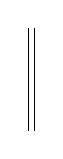
\begin{tikzpicture}\draw (0,0)--(0,1.3);\draw (.08,0)--(.08,1.3);\end{tikzpicture}}}
cette donnée (22) \unsure{ne peut en aucun cas} décrire $\varphi$ lui-même, mais seult
$\varphi|\widetilde{\mathbb Q}$.
Mais je pense que la conn. de \deleted{$\unsure{\varphi}$} $P_{X,x}^{\varphi}$
(ou $Q_X^{\varphi}$) lui-même, pour tt $X$ (et tt $g,\nu$) définit $\varphi$\ldots
\mspage{17}

\scanpage{19}
\mspage{4)}
Récapitulation (II)

$k$ corps \uline{alg. clos}, car. 0 i.e. \deleted{\unsure{k}} $\mathbb Q\longrightarrow k$,
$X$ courbe de type $g,\nu$ sur $k$, $x\in X$ ; d'où
\[
\xi\in\deleted{\unsure{\mathrm{Pt}}}M_{g,\nu}(k)=\uline{\Gamma}(M_{g,\nu\,k}/k)
\qquad X=\mathcal X_{g,\nu\,\xi}=(\mathcal X_{g,\nu\,k})_\xi
\]
\[x\in\mathcal X_{g,\nu}(k)\]
$\xi,x$ pts géométriques de $M_{g,\nu\,\mathbb Q},\mathcal X_{g,\nu\,\mathbb Q}$,
d'où par fibration double
\[
(0)\quad\left\{\diagram{\begin{tikzcd}
\mathcal X_{g,\nu\,\mathbb Q}\arrow[r,no head]\arrow[d]&\mathcal X_{g,\nu\,k}\arrow[d,no head]\\
M_{g,\nu\,\mathbb Q}\arrow[d,no head]&M_{g,\nu\,k}\arrow[d,no head]\\
\mathbb Q\arrow[r,no head]&k
\end{tikzcd}}\right.
\]
le diagramme de suites exactes
\diagram{\begin{tikzcd}
&1\arrow[d]&1\arrow[d]&&\\
&\Pi_{X,x}\arrow[r,Rightarrow]\arrow[d]&\unsure{\Gamma_{X,x}|\Pi_{X,x}}\arrow[d]\arrow[r,no head]&{}&\\
1\arrow[r]&\mathcal G_{X,x}\arrow[r]\arrow[d]&\mathcal M_{X,x}\arrow[r]\arrow[d]&\Gamma_{\widetilde{\mathbb Q}/\mathbb Q}\arrow[r,no head]\arrow[d,equal]&1\\
1\arrow[r]&\Gamma_X\arrow[r]\arrow[d]&\mathcal N_{X\deleted{,x}}\arrow[r,no head]\arrow[d]&\Gamma_{\widetilde{\mathbb Q}/\mathbb Q}\arrow[r,no head]\arrow[d,no head]&1\\
&1&1&\unsure{1}&
\end{tikzcd}}
\margin{(1)}
\margin{$\widetilde{\mathbb Q}$ est la clôture alg. de $\mathbb Q$ dans $k$}
\margin{\uline{NB} Ce diagramme équivaut à la donnée de
\[
1\subset\overbrace{\underbrace{\Pi_{X,x}\subset\mathcal G_{X,x}}_{\Gamma_X}
\underbrace{{}\subset\mathcal M_{X,x}}_{\deleted{\unsure{\mathcal N}}\Gamma_{\widetilde{\mathbb Q}/\mathbb Q}}}^{\mathcal N_X}
\]}
où \deleted{$\unsure{\mathcal G_{X,x}\text{ est}}$}
\[
(2)\quad\mathrm{déf}\left\{\begin{aligned}
\Pi_{X,x}&=\pi_1(X,x) &&(\simeq\widehat\Pi_{g,\nu}\text{ non cant.})\\
\unsure{\mathcal G_{X,x}}&=\pi_1(\mathcal X_{g,\nu\,k},x)&&(\simeq\widehat{\mathcal G}_{g,\nu}\text{ ---})\\
\Gamma_X&=\pi_1(M_{g,\nu\,k},\xi)&&(\simeq\widehat\Gamma_{g,\nu}\ \ldots)\\
\mathcal M_{X,x}&=\pi_1(\unsure{\mathcal X_{g,\nu}|M_{g,\nu}},\deleted{\xi}\inserted{x})&&(\simeq\mathcal M_{g,\nu}\ \ldots)\\
\mathcal N_X&=\pi_1(M_{g,\nu},\xi)&&(\simeq\mathcal N_{g,\nu}\ \ldots)
\end{aligned}\right.
\]
Les deuxièmes mb $\widehat\Pi_{g,\nu}$ se définissent comme les premiers,
mais à l'aide de $(X_0,x_0)$ sur $\mathbb C$, de type $g,\nu$,
définissant les pts géom. $x_0$ et $\xi_0$ de
$\mathcal X_{g,\nu\,\mathbb Q}$ et $M_{g,\nu\,\mathbb Q}$.
\mspage{18}

\scanpage{20}
Les \unsure{choix|classes} de chemins de $\unsure{\xi_0|x_0}$ à $\unsure{\xi|x}$
définissent un torseur
\[
(3)\qquad P_{X,x}\quad\text{torseur à droite sous }\mathcal M_{g,\nu}
\quad\begin{gathered}(\text{\unsure{commutant}}\ \mathcal M_{X,x})\end{gathered}
\]
de telle façon que (1) soit déduit du diagramme analogue pour $(X_0,x_0)$
\[
(1_{g,\nu})\qquad
\diagram{\begin{tikzcd}
&1\arrow[d]&1\arrow[d]&&\\
&\widehat\Pi_{g,\nu}\arrow[r,equal]\arrow[d]&\widehat\Pi_{g,\nu}\arrow[d]&&\\
1\arrow[r,no head]&\widehat{\mathcal G}_{g,\nu}\arrow[r,no head]\arrow[d]&\mathcal M_{g,\nu}\arrow[r,no head]\arrow[d]&\Gamma_{\overline{\mathbb Q}/\mathbb Q}\arrow[r,no head]\arrow[d,equal]&1\\
1\arrow[r,no head]&\widehat\Gamma_{g,\nu}\arrow[r,no head]\arrow[d]&\mathcal N_{g,\nu}\arrow[r,no head]\arrow[d]&\Gamma_{\overline{\mathbb Q}/\mathbb Q}\arrow[r,no head]&1\\
&1&1&&
\end{tikzcd}}
\]
en le tordant, grâce à l'action de $\mathcal M_{g,\nu}$ opérant par autom. int.
sur lui-même, et sur sa filtration par $\widehat{\mathcal G}_{g,\nu},\widehat\Pi_{g,\nu}$.
En particulier
\[
(4)\quad\left\{\begin{aligned}
\Pi_{X,x}&\simeq P_{X,x}\wedge_{\mathcal M_{g,\nu}}\widehat\Pi_{g,\nu}\\
\mathcal G_{X,x}&\simeq P_{X,x}\wedge_{\mathcal M_{g,\nu}}\widehat{\mathcal G}_{g,\nu}
\qquad\deleted{\mathcal M_{X,x}}\\
\Gamma_{X,x}&\simeq P_{X,x}\wedge_{\mathcal M_{g,\nu}}\widehat\Gamma_{g,\nu}
\simeq\unsure{Q_X|Q_{X_0}}\wedge_{\mathcal N_{g,\nu}}\widehat\Gamma_{g,\nu}\\
\mathcal M_{X,x}&\simeq P_{X,x}\wedge_{\mathcal M_{g,\nu}}\mathcal M_{g,\nu}\\
\mathcal N_X&\simeq P_{X,x}\wedge_{\mathcal M_{g,\nu}}\mathcal N_{g,\nu}
\simeq Q_X\wedge_{\mathcal N_{g,\nu}}\mathcal N_{g,\nu}\\
\widetilde{\mathbb Q}&\simeq P_{X,x}\wedge_{\mathcal M_{g,\nu}}\overline{\mathbb Q}
\simeq Q_X\wedge_{\mathcal N_{g,\nu}}\overline{\mathbb Q}
\simeq R\wedge_{\Gamma_{\overline{\mathbb Q}/\mathbb Q}}\overline{\mathbb Q}
\end{aligned}\right.
\]
\mspage{19}

\scanpage{21}
\mspage{5)}
où
\[
(5)\quad Q_X=P_{X,x}\wedge_{\mathcal M_{g,\nu}}\mathcal N_{g,\nu},\qquad
R=P_{X,x}\wedge_{\mathcal M_{g,\nu}}\Gamma_{\overline{\mathbb Q}/\mathbb Q}
\simeq Q_X\wedge_{\mathcal N_{g,\nu}}\Gamma_{\overline{\mathbb Q}/\mathbb Q}
\]
Ainsi, $\widetilde{\mathbb Q}$ et (1) sont connus par la connaissance du
\inserted{$\mathcal M_{g,\nu}$-tors. $P_{X,x}$} (3). Mais bien sûr même si
$k$ est alg. sur $\mathbb Q$ ($k=\widetilde{\mathbb Q}$, voire $k=\overline{\mathbb Q}$
i.e. \unsure{avec} $R$ trivialisé) la donnée de \deleted{\unsure{Q}} $P_{X,x}$
ne permet pas de récupérer $X$ sur $k$ --- p.ex. les autom. du torseur $P_{X,x}$
sont les élémts de $\mathcal M_{X,x}$ --- ils ont la puissance du continu ---
ceux du \deleted{\unsure{Q}} $\widehat{\mathcal G}_{g,\nu}$-torseur correspondant
à une restriction du groupe structural à $\widehat\Gamma_{g,\nu}$ i.e. à
un iso. $\widetilde{\mathbb Q}\simeq\overline{\mathbb Q}$, correspondent aux
éléments de $\widehat{\mathcal G}_{X,x}$ --- il a la puissance du continu,
tandis que les autom. de $X,x$ compatibles avec l'identité sur
$k=\widetilde{\mathbb Q}$ ($\overset{\mathrm{donné}}\simeq\overline{\mathbb Q}$)
font un groupe \uline{fini} !

Mais\ldots
\[
(6)\qquad k=\underset{i}{\uline{\lim}}\ K_i
\]
les $K_i$ sous-corps de t.f. --- et \deleted{\unsure{une}}\inserted{la}
structure etc $(X,x)$ implique une structure
\mspage{20}

\scanpage{22}
``définie sur $K_i$ pour $i$ assez grand''.
Choisissons un tel $K=K_i$, et essayons d'exprimer l'information supplémentaire
de type ``galoisien'' \unsure{qui l'exprime|qu'il exprime}. Soit $\overline K$ la clôture alg.
de $K$ dans $k$. Considérons
\[
(7)\quad\diagram{\begin{tikzcd}[column sep=large]
\mathcal X_{g,\nu\,\mathbb Q}\arrow[d]&\mathcal X_{g,\nu\,K}\arrow[l]\arrow[d,no head]&\mathcal X_{g,\nu\,\overline K}\arrow[l,no head]\arrow[d,no head]&\mathcal X_{g,\nu\,k}\arrow[l,no head]\arrow[d,no head]\\
M_{g,\nu\,\mathbb Q}\arrow[d]&M_{g,\nu\,K}\arrow[l]\arrow[d,no head]&M_{g,\nu\,\overline K}\arrow[l,no head]\arrow[d,no head]&M_{g,\nu\,k}\arrow[l,no head]\arrow[d,no head]\\
\mathbb Q&K\arrow[l,no head]\arrow[u,dashed,bend right=35]\arrow[uu,dashed,bend right=55]&\overline K\arrow[l,no head]&k\arrow[l,no head,"{\underbrace{\hspace{2.3cm}}_{\substack{\text{du pt de vue}\\\text{homotopique, cette}\\\text{extension est de}\\\text{nature triviale}}}}"']
\end{tikzcd}}
\]
$(X,x)$ provient d'une \deleted{\unsure{pt}}\inserted{section} (notée encore $x$)
de $\unsure{\mathcal X_{g,\nu\,K}|M_{g,\nu\,K}}$ sur $K$, définissant une section
(notée encore $\xi$) de $M_{g,\nu\,K}$ sur $K$, (dont sont déduites les sections
$x,\xi$ sur $k$, par changement de corps de base).

Posons
\[
(\unsure{8})\quad\left\{\begin{aligned}
\mathcal M_{X,x,K}&=\pi_1(\unsure{\mathcal X_{g,\nu\,K}|M_{g,\nu\,K}},\deleted{\xi}\inserted{x})\\
\mathcal N_{X,x,K}&=\pi_1(M_{g,\nu\,K},\xi)\\
\Gamma_{\overline K/K}&=\operatorname{Gal}(\overline K/K)=\pi_1(\operatorname{Spec}K,\unsure{\overline K|\overline k})
\end{aligned}\right.
\]
on a cette fois-ci, comme (1) avec $K$ remplaçant $\mathbb Q$ :
\mspage{21}

\scanpage{23}
\mspage{6)}
\[
(9)\quad\diagram{\begin{tikzcd}
&1\arrow[d]&1\arrow[d]&&\\
&\Pi_{X,x}\arrow[r,equal]\arrow[d]&\Pi_{X,x}\arrow[d]&&\\
1\arrow[r,no head]&\mathcal G_{X,x}\arrow[r,no head]\arrow[d,no head]&\mathcal M_{X,x\,K}\arrow[r,no head]\arrow[d]&\Gamma_{\overline K/K}\arrow[r,no head]\arrow[d,equal]&1\\
1\arrow[r,no head]&\Gamma_X\arrow[r,no head]\arrow[d]&\mathcal N_{X,x\,K}\arrow[r,no head]\arrow[d]&\Gamma_{\overline K/K}\arrow[r,no head]&1\\
&1&1&&
\end{tikzcd}}
\]
correspondant à
\[
(10)\qquad\overbrace{\underbrace{\Pi_{X,x}\subset\mathcal G_{X,x}}_{\Gamma_X}
\underbrace{{}\subset\mathcal M_{X,x,K}}_{\Gamma_{\overline K/K}}}^{\mathcal N_{X,K}}
\]
(\uline{NB} On n'a pas encore utilisé que $(X,x)$ soit défini sur $K$, i.e. que
$x$ \inserted{$(\in\mathcal X_{g,\nu}(k))$} provienne d'un pt à val. dans $K$\ldots).
À vrai dire, la situation (9) \inserted{ou (10)} se déduit de la situation
``absolue'' (i.e. sur $\mathbb Q$) (1), par \unsure{la|le} image inverse de structures
d'extensions (de $\Gamma_{\widetilde{\mathbb Q}/\mathbb Q}$ par
$\mathcal G_{X,x}\supset\Pi_{X,x}$) à l'aide de l'hom. de groupes
\[
(11)\qquad\Gamma_{\overline K/K}\longrightarrow\Gamma_{\widetilde{\mathbb Q}/\mathbb Q}
\]
\mspage{22}

\scanpage{24}
par
\[
(12)\quad\left\{\begin{aligned}
\mathcal M_{X,x,K}&\simeq\mathcal M_{X,x}\times_{\Gamma_{\widetilde{\mathbb Q}/\mathbb Q}}\Gamma_{\overline K/K}\\
\mathcal N_{X,x,K}&\simeq\mathcal N_{X,x}\times_{\Gamma_{\widetilde{\mathbb Q}/\mathbb Q}}\Gamma_{\overline K/K}
\end{aligned}\right.
\]
\deleted{\unsure{d'où}}\inserted{i.e.}
\[
(13)\quad\diagram{\begin{tikzcd}
1\arrow[r,no head]&\mathcal G_{X,x}\arrow[r,no head]&\mathcal M_{X,x}\arrow[r,no head]&\Gamma_{\widetilde{\mathbb Q}/\mathbb Q}\arrow[r,no head]&1\\
1\arrow[r,no head]&\mathcal G_{X,x}\arrow[u,equal]\arrow[r,no head]&\mathcal M_{X,x,K}\arrow[u]\arrow[r,no head]\arrow[ur,phantom,"\text{cart}" description]&\Gamma_{\overline K/K}\arrow[u]\arrow[r,no head]&1
\end{tikzcd}}
\]
et de même
\[
(13')\quad\diagram{\begin{tikzcd}
1\arrow[r,no head]&\unsure{\Gamma_{X,x}}\arrow[r,no head]&\mathcal N_{X,x}\arrow[r,no head]&\Gamma_{\widetilde{\mathbb Q}/\mathbb Q}\\
1\arrow[r,no head]&\Gamma_{X,x}\arrow[u,equal]\arrow[r,no head]&\unsure{\mathcal N_{X,x,K}|\mathcal M_{X,x,K}}\arrow[u]\arrow[r,no head]\arrow[ur,phantom,"\text{cart}" description]&\Gamma_{\overline K/K}\arrow[u]
\end{tikzcd}}
\]
(déduit du précédent en divisant par $\Pi_{X,x}\subset\mathcal G_{X,x}$)

Ceci posé, la donnée de la section $x$ de
$\unsure{\mathcal X_{g,\nu\,K}|M_{g,\nu\,K}}$ sur $K$ définissant $x$ sur $k$
(i.e. de la restriction du corps de base de $k$ à $K$ dans $(X,x]$)
s'exprime par un scindage \inserted{can.} de l'ext. $\mathcal M_{X,x,K}$,
\mspage{23}

\scanpage{25}
\mspage{8)}
ou encore par un relèvement
\[
(14)\quad\diagram{\begin{tikzcd}
\mathcal M_{X,x}\arrow[r,no head]&\Gamma_{\widetilde{\mathbb Q}/\mathbb Q}\\
&\Gamma_{\overline K/K}\arrow[u]\arrow[ul,dashed]
\end{tikzcd}}
\]
et de même pour $\xi$, correspondant à une restriction du corps de définition
$k$ de $X$ à $K$, ceci correspond à
\[
(14')\quad\diagram{\begin{tikzcd}
\mathcal N_{X,x}\arrow[r,two heads]&\Gamma_{\widetilde{\mathbb Q}/\mathbb Q}\\
&\Gamma_{\overline K/K}\arrow[u]\arrow[ul,dashed]
\end{tikzcd}}
\]
\deleted{\unsure{La donnée donc, puisque}}

\margin{\figure{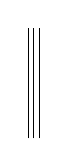
\begin{tikzpicture}\draw (0,0)--(0,1.4);\draw (.07,0)--(.07,1.4);\draw (.14,0)--(.14,1.4);\end{tikzpicture}}}
Je pense que ces données permettent de réconstituer $(K,\overline K,(X,x))$
resp $(K,\overline K,X)$.

J'ai envie d'exprimer la structure de façon plus simple, en notant que (14)
\inserted{resp $(14')$} implique
\[
(15)\qquad\Gamma_{\overline K/K}\longrightarrow\operatorname{Aut}_{\mathrm{loc}}\Pi_{X,x}
\qquad\text{resp.}
\]
\[
(15')\qquad\Gamma_{\overline K/K}\mathbin{-}\operatorname{Autext}_{\mathrm{loc}}(\Pi_{X,x})
\]
\mspage{24}

\scanpage{26}
J'ai envie d'abord de montrer comment ces données,
\deleted{\unsure{à priori de deux grs}} (d'un
$\Gamma=\Gamma_{\overline K/K}$, avec hom ext dans
$\Gamma_{\overline{\mathbb Q}/\mathbb Q}\overset{\text{non can!}}\simeq
\Gamma_{\widetilde{\mathbb Q}/\mathbb Q}$),
$\Gamma$ opérant sur un groupe profini à la $\Pi_{X,x}$) permettent, à peu de
choses près, de réconstituer ces \unsure{mach.}.
\deleted{Notons que}\inserted{Il faut de plus} se donner une
\uline{arithmétisation} de $\Pi_{X,x}$,
\deleted{l'image de $\Gamma_{\overline K/K}$ \unsure{et}}
stable par l'action de $\Gamma$, i.e. un paquet de discrétisations
\deleted{de} formant un torseur sous
$\mathcal M_{g,\nu}'\subset\operatorname{Aut}_{\mathrm{loc}}(\widehat\Pi_{g,\nu})$.
Cela donne tout au moins le torseur sous $\mathcal M_{g,\nu}'$
(voire sous $\mathcal M_{g,\nu}$), ou (dans le cas $(15')$) le torseur sous
$\mathcal N_{g,\nu}'$ --- qui sont des quotients de $\mathcal M_{g,\nu}$
resp. $\mathcal N_{g,\nu}$.
\mspage{25}

\scanpage{27}
$K$ corps de t.f. sur $\mathbb Q$

$\overline K$ clôture algébrique.

$D$-structure sur $\overline K$ :
\[
\left\{\begin{array}{ll}
\text{a)}&\overline{\mathbb Q}\subset\overline K\\
\text{b)}&\text{pour tt courbe alg. }X\text{ sur }\overline K\text{ de type }g,\nu,
\end{array}\right.
\]
la donnée d'une discrétification de $\pi_1(X)$

$D$ structure \inserted{spéciale} \unsure{si possible} par plongt
$\varphi:\overline K\longrightarrow\mathbb C$

\deleted{\uline{Prop.} Soient $\Theta,\Theta'$ deux}

Soient $\overline K,\overline K'$ deux clôtures algébriques.
Pour tt \deleted{\unsure{K}} $K$-isom (plus gén, pour tt isom)
$\overline K\mathbin{-}\overline K'$, par transport de structure une $D$ structure
(resp. spéciale) sur $\overline K$ en définit une sur $\overline K'$.
En particulier, $\Gamma=\operatorname{Aut}(\overline K/K)$ opère sur l'ens des
discrétifications (resp. spéciales) de $\overline K$.

\uline{Prop} Soient $\overline K,\overline K'$ deux clôtures algébriques de $K$,
munies de discret. \uline{spéciales} $\Theta,\Theta'$. Alors il existe un
$K$-isom $\overline K\mathbin{-}\overline K'$ compatible avec $\Theta,\Theta'$.

\uline{Cor} Deux discrétifications spéciales sur $\overline K$ sont isomorphes
par un élémnt de $\Gamma=\operatorname{Aut}_K(\overline K)$ (et même, par un élémnt
d'un sous-groupe d'indice fini \inserted{donné} de $\Gamma$).

\uline{NB}
\diagram{\begin{tikzcd}[column sep=small]
\operatorname{Isom}_{\deleted{K}}(\overline K,\overline K')\arrow[d,phantom]&{}
\times\operatorname{Discr}(\overline K)&\operatorname{Discr}(\overline K')\\
\operatorname{Isom}_K(\overline K,\overline K')\arrow[u]&{}
\times\operatorname{Hom}(\overline K,\mathbb C)\arrow[u]\arrow[r,no head]&\operatorname{Hom}(\overline K',\mathbb C)\arrow[u]
\arrow[from=1-2,to=1-3,no head]
\end{tikzcd}}
\margin{!\quad\figure{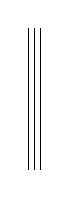
\begin{tikzpicture}\draw (0,0)--(0,1.8);\draw (.08,0)--(.08,1.8);\draw (.16,0)--(.16,1.8);\end{tikzpicture}}}
\deleted{\unsure{on tire}}\inserted{est} \unsure{le|un} commutatif.
\deleted{\unsure{$\overline K\subset\mathbb C$}}
Si $\overline K=\overline K'$, alors on se limite à
$\operatorname{Isom}_K(\overline K,\overline K')=\Gamma$ : --- \unsure{voir l'append.|cf. l'append.}
\mspage{26}

\scanpage{28}
\margin{\figure{\begin{tikzpicture}\draw (0,.2)--(.25,0)--(.55,.35);\end{tikzpicture}}}
\margin{\uline{Soit}\quad Soit \uline{alors}}
\[
\operatorname{Hom}(\overline K,\mathbb C)\xrightarrow{\mathrm{surj}}
\operatorname{Discspec}(\overline K)
\]
est \deleted{\illegible{1}} compatible avec les op. naturelles de $\Gamma$.
\margin{\figure{\begin{tikzpicture}\draw (0,0)--(0,1);\draw (.07,0)--(.07,1);\end{tikzpicture}}}
\deleted{\unsure{Et pour cela}}\inserted{NB} $\Gamma$ est transitif à
\deleted{gauche}\inserted{droite}, et évidemment non transitif à
\deleted{droite}\inserted{gauche}$^*$ (pour que
$\varphi,\varphi':\overline K\rightrightarrows\mathbb C$ soient conjugués par $\Gamma$,
il faut que a) $\varphi|K=\varphi'|K$ et b)
$\varphi(\overline K)=\varphi'(\overline K)$), conditions qui sont des plus
\unsure{draconiennes}\ldots
\margin{$^*$ sauf si $\overline K=\overline{\mathbb Q}$ ($K$ alg. sur $\mathbb Q$
i.e. fini sur $\mathbb Q$)}
\margin{\uline{\unsure{donc les flèches}}\quad\uuline{\unsure{rien}}\quad\uline{\unsure{d'injectif}}}

\uline{\unsure{Autos}} d'une discrétification sur $\overline K$ : on en trouve
d'intéressants par \deleted{\unsure{les}} des
\deleted{\unsure{chemins}}\inserted{``éléments} transcendants'' sur
$K\otimes_{\mathbb Q}\mathbb C$,\ldots\deleted{\unsure{\ldots}}

Est-il possible que $\operatorname{Hom}(\overline K,\mathbb C)\longrightarrow
\operatorname{Discspec}(\overline K)$ soit injectif (i.e bijectif) ?
\deleted{\unsure{Si c'était le cas donc la donnée de}
$\overline K\subset\mathbb C$ \unsure{resp.}}
\inserted{$(K,\overline K,\overline K\xrightarrow{\varphi_{\overline K}}\mathbb C)$}
\deleted{\unsure{resp.}}
i.e. de $(K,\varphi_K:K\mathbin{-}\mathbb C)$, \uline{équivalant} à celle
de $(K,\overline K,\Theta)$ \inserted{$\Theta=\Theta_{\varphi_{\overline K}}$},
\deleted{et tt \unsure{sans autre rigidifications}}
\unsure{Seulement dans le cas trivial} où $\unsure{K|\widehat K}$ est alg. sur $\mathbb Q$.

$\Pi_1\quad\Pi_{1\,\mathrm{ab}}^{\deleted{\unsure{\circ}}}$\quad
\uline{structure de Hodge mixte}
\[
\Pi_{1\,\mathrm{ab}}\otimes_{\mathbb Z}\mathbb C
\]
ou encore structure complexe sur $\unsure{\widetilde\Pi_{1\,\mathrm{ab}}|\Pi_{1\,\mathrm{ab}}}\otimes_{\mathbb Z}\mathbb R$
\mspage{27}

\scanpage{29}
Formulaire pour $\Pi_{0,3}$ etc

Pt de vue transcendant pour $M_{1,1}$
\mspage{28}

\scanpage{30}
\uline{$\mathrm{GL}(2,\mathbb Z)$}\qquad (Formulaire $2^e$ version)\qquad (1982)
\margin{\figure{\begin{tikzpicture}\draw[->] (.6,0) .. controls (-.5,.3) and (-.5,1.5) .. (.5,1.8);\end{tikzpicture}}}
\[
\boxed{\rho=\begin{pmatrix}0&1\\-1&1\end{pmatrix}},\qquad
\rho^{-1}=\begin{pmatrix}1&-1\\1&0\end{pmatrix}
\]
\[
\rho^3=\rho^{-3}=\omega\qquad\text{donc }\rho^2=\omega\rho^{-1}
\qquad\rho^6=1
\]
\[
\omega=\begin{pmatrix}-1&0\\0&-1\end{pmatrix}\quad(\text{donc }\omega g=-g)
\qquad\omega^2=1\quad\deleted{\unsure{\Rightarrow}}
\]
\[
\left\{\begin{aligned}
\boxed{\sigma_\infty=\begin{pmatrix}0&1\\-1&0\end{pmatrix}}\\
\sigma_0=\begin{pmatrix}-1&1\\-2&1\end{pmatrix}\\
\sigma_1=\begin{pmatrix}-1&2\\-1&1\end{pmatrix}
\end{aligned}\right.
\qquad
\begin{gathered}
\sigma_\infty^{-1}=\omega\sigma_\infty=\begin{pmatrix}0&-1\\1&0\end{pmatrix}\\
\sigma^2=\sigma^{-2}=\omega,\quad\sigma^{-1}=\omega\sigma\\
\rho(\sigma_i)=\sigma_{i+1}\qquad\sigma_i^2=\omega,\quad\sigma_i^{-1}=\omega\sigma_i
\end{gathered}
\]
\[
\left\{\begin{aligned}
\boxed{\varepsilon_0=\sigma_\infty^{-1}\rho=\begin{pmatrix}1&-1\\0&1\end{pmatrix}}\\
\boxed{\varepsilon_1=\rho\sigma_\infty^{-1}=\begin{pmatrix}1&0\\1&1\end{pmatrix}}\\
\varepsilon_\infty=\rho^2\sigma_\infty^{-1}\rho^{-1}=\begin{pmatrix}2&-1\\1&0\end{pmatrix}
\end{aligned}\right.
\qquad(\uline{unipotent}\ \deleted{\unsure{\&}}\ \uline{\unsure{réguliers}})
\]
\margin{\[
\left\{\begin{aligned}
N_0&=\begin{pmatrix}0&-1\\0&0\end{pmatrix}\\
N_1&=\begin{pmatrix}0&0\\1&0\end{pmatrix}\\
N_\infty&=\begin{pmatrix}1&-1\\1&-1\end{pmatrix}
\end{aligned}\right.
\]}
\[
\left\{\begin{aligned}
\rho_0&=\varepsilon_0^2=\begin{pmatrix}1&-2\\0&1\end{pmatrix}\\
\rho_1&=\varepsilon_1^2=\begin{pmatrix}1&0\\2&1\end{pmatrix}\\
\rho_\infty&=\varepsilon_\infty^2=\begin{pmatrix}3&-2\\2&-1\end{pmatrix}
\end{aligned}\right.
\]
\[
\deleted{\unsure{\rho(\varepsilon_i)=\varepsilon_{i+1}}}\qquad
\varepsilon_i=\sigma_i^{-1}\rho\qquad
\rho(\varepsilon_i)=\varepsilon_{i+1}\qquad\rho(\rho_i)=\rho_{i+1}
\]
\[
\rho_\infty\rho_1\rho_0=\omega\qquad
\rho'_\infty\rho'_1\rho'_0=1\quad\text{où }\rho'_i=\omega\rho_i
\]
\[
\left\{\begin{aligned}
\sigma_i\sigma_{i+1}&=\omega\rho\rho_i=\omega\rho_{i+1}\rho\\
\rho(\sigma_i)&=\sigma_{i+1}=\omega\unsure{\rho'_{i-1}|\rho_{i-1}}\varepsilon_{i+1}\\
\sigma_i(\rho)&=\rho^{-1}\rho'_{i-1}
\end{aligned}\right.
\]
\[
\left\{\begin{aligned}
\boxed{\tau_\infty=\begin{pmatrix}-1&0\\0&+1\end{pmatrix}}\\
\tau_0=\begin{pmatrix}1&0\\2&-1\end{pmatrix}\\
\tau_1=\begin{pmatrix}1&-2\\0&-1\end{pmatrix}
\end{aligned}\right.
\qquad
\begin{gathered}
\tau_i^2=1\qquad\rho(\tau_i)=\tau_{i+1}\\
\tau_i\tau_{i-1}=\underbrace{\omega\rho_{i+1}}_{\rho'_{i+1}}\quad\text{i.e. }
\left\{\begin{aligned}
\tau_1\tau_0&=\deleted{\omega}\rho'_\infty\\
\tau_\infty\tau_1&=\deleted{\omega}\rho'_0\\
\tau_0\tau_\infty&=\deleted{\omega}\rho'_1
\end{aligned}\right.
\end{gathered}
\]
\[
\left\{\begin{aligned}
\boxed{\tau'_\infty=\sigma_\infty\tau_\infty=\omega\tau_\infty\sigma_\infty=\begin{pmatrix}0&1\\1&0\end{pmatrix}}\\
\tau'_0=\sigma_0\tau_0=\omega\tau_0\sigma_0=\begin{pmatrix}1&-1\\0&-1\end{pmatrix}\\
\tau'_1=\sigma_1\tau_1=\omega\tau_1\sigma_1=\begin{pmatrix}-1&0\\-1&1\end{pmatrix}
\end{aligned}\right.
\]
\[
\unsure{(\tau'_i)^2}=1\qquad\rho(\tau'_i)=\tau'_{i+1}
\]
\[
\begin{aligned}
\tau'_0\tau'_1&=\tau'_1\tau'_\infty=\tau'_\infty\tau'_0=\deleted{\unsure{\omega}}\rho\\
\tau'_1\tau'_0&=\tau'_\infty\tau'_1=\tau'_0\tau'_\infty=\omega\rho^{-1}\\
\tau'_i&=\sigma_i\tau_i=\omega\tau_i\sigma_i=\tau_i\sigma_i^{-1}\\
\tau_i&=\tau'_i\sigma_i=\omega\sigma_i\tau'_i=\sigma_i^{-1}\tau'_i\\
\unsure{\sigma_i}&=\unsure{\tau'_i\tau_i}=\unsure{\omega\tau_i\tau'_i}
\end{aligned}
\]
\mspage{29}

\scanpage{31}
\[
\left\{\begin{gathered}
\left.\begin{aligned}
\tau_i(\varepsilon_j)&=\varepsilon_j^{-1}\\
\tau_i(\rho_j)&=\rho_j^{-1}\\
\tau_i(\rho'_j)&=(\rho'_j)^{-1}
\end{aligned}\right|\ \text{si }i\ne j\\[4pt]
\left\{\begin{aligned}
\tau_i(\sigma_i)&=\inserted{\tau'_i(\sigma_i)=}\sigma_i^{-1}=\omega\sigma_i\\
\tau'_i(\rho)&=\rho^{-1}\\
\tau_i(\rho)&=(\rho'_{i-1})^{-1}\rho=\sigma_i(\rho^{-1})
\end{aligned}\right.
\end{gathered}\right.
\]
\[
\deleted{\unsure{\tau_i(\varepsilon_i)=}}\quad
\begin{aligned}
\tau_\infty(\varepsilon_0)&=\varepsilon_0^{-1}\\
\tau_\infty(\varepsilon_1)&=\varepsilon_1^{-1}\\
\tau_\infty(\varepsilon_\infty)&=\rho_0(\varepsilon_\infty^{-1})
=\rho_1^{-1}(\varepsilon_\infty^{-1})
\end{aligned}
\qquad
\begin{aligned}
\tau_\infty(\rho_0)&=\rho_0^{-1}\\
\tau_\infty(\rho_1)&=\rho_1^{-1}\\
\tau_\infty(\rho_\infty)&=\rho_0\rho_1\omega\\
&=\rho_1^{-1}(\rho_\infty^{-1})\unsure{\omega}\\
&=\rho_0(\rho_\infty^{-1})\deleted{\unsure{\omega}}
\end{aligned}
\]
\[
\begin{aligned}
\sigma_i(\rho_{i+1})&=\rho_{i+2}&\quad\sigma_i(\varepsilon_{i+1})&=\varepsilon_{i+2}\\
\sigma_i(\rho_{i+2})&=\rho_{i+1}&\sigma_i(\varepsilon_{i+2})&=\varepsilon_{i+1})\\
\sigma_i(\rho_i)&=\underbrace{\omega(\rho_{i+1}\rho_{i+2})^{-1}}_{\omega\rho_{i+2}^{-1}\rho_{i+1}^{-1}}
=\rho_{i+1}(\rho_i)=\rho_{i+2}^{-1}(\rho_i)
\end{aligned}
\]
\[\mathbin{---}\]
\[
\left\{\begin{gathered}
\deleted{\unsure{\rho}}\lambda_0=\varepsilon_0,\quad\lambda_1=\sigma_\infty,
\quad\lambda_\infty=\rho^{-1}\\
\lambda_\infty\lambda_1\lambda_0=1\qquad\lambda_1^4=\lambda_\infty^6=1
\end{gathered}\right.
\]
\[
r_0=\tau'_\infty\inserted{=\begin{pmatrix}0&1\\1&0\end{pmatrix}},\quad
r_1=-\tau'_0\inserted{=\begin{pmatrix}-1&1\\0&1\end{pmatrix}},\quad
r_\infty=\tau_\infty\inserted{\left(=\begin{pmatrix}-1&0\\0&1\end{pmatrix}\right)}
\]
\[
\begin{aligned}r_\infty r_1&=\lambda_0\\r_0r_\infty&=\lambda_1\\r_1r_0&=\lambda_\infty\end{aligned}
\]
donc on a
\diagram{\begin{tikzcd}
\Pi_{0,3}^{\tau}\arrow[r,"\varphi"]\arrow[d,hook]&\mathrm{GL}(2,\mathbb Z)\arrow[d,hook]\\
\Pi_{0,3}\arrow[r,"\varphi^0"]&\mathrm{SL}(2,\mathbb Z)
\end{tikzcd}}
\[\varphi,\varphi^0\ \uline{\text{surj.}}\qquad
\varphi(\rho_i)=\lambda_i\qquad\varphi(\tau_i)=r_i\]
\margin{$\sigma=\sigma_\infty$\qquad$\tau'=\tau'_\infty$}
\[
\mathrm{SL}(2,\mathbb Z)=\{\rho,\sigma\mid\rho^3=\rho^{-3}=\sigma^2\ (=\sigma^{-2})\}
=\mathbb Z/6\mathbb Z*_{\mathbb Z/2\mathbb Z}\mathbb Z/4\mathbb Z
\]
\[
\begin{aligned}
\mathrm{GL}(2,\mathbb Z)&=\{\rho,\sigma,\tau'_\infty\mid
\rho^3=\rho^{-3}=\sigma^2\ (=\sigma^{-2}),\
\tau'(\rho)=\rho^{-1},\ \tau'(\sigma)=\sigma^{-1}\}\\
&=\{r_0,r_1,r_\infty\mid r_0^2=r_1^2=r_\infty^2=1,\
(r_0r_\infty)^2=(r_1r_0)^3=(r_1r_0)^{-3}\}\\
&=D_6*_{D_2}D_4
\end{aligned}
\]
\margin{\[
\left\{\begin{gathered}
\mathrm{NB}\quad\tau'=r_0,\ \deleted{\unsure{\rho}}\quad r_0(\rho)=\rho^{-1}\\
r_0(\sigma)=\sigma^{-1}\\
\deleted{\unsure{\sigma_0}}\quad r_1=\rho^{-1}r_0=r_0\rho\\
r_\infty=\sigma r_0=r_0\sigma^{-1}
\end{gathered}\right.
\]}
\uline{Relations avec le formulaire 1981}

Les $\sigma_i$ sont transformés en $\sigma_i^{-1}$, donc
$\varepsilon_0=\unsure{\sigma_i^{-1}|\sigma_\infty^{-1}}\rho$ au lieu de
$\varepsilon_0=\unsure{\sigma_i|\sigma_\infty}\rho$.
Les autres quantités pas changées, mais on écrit $\rho_i=\varepsilon_i^2$
au lieu de $\unsure{h_i|\ell_i}$, et
$\rho'_i=\omega\varepsilon_i^2=\omega\rho_i$ au lieu de $\lambda_i$.
($\rho'_\infty\rho'_1\rho'_0=1,\ \rho_\infty\rho_1\rho_0=\omega$), où
$\omega=-\mathrm{id}$. Les $\unsure{\ell'_i|h'_i}$ sont devenus $\lambda_i$.
\mspage{30}

\scanpage{32}
\margin{(1982)}
\diagram{\begin{tikzcd}1\arrow[r,dash]&\mathbb Z\arrow[r,"\kappa"]&GL(2,\mathbb Z)^{\sim}\arrow[r]&GL(2,\mathbb Z)\arrow[r]&1\end{tikzcd}}
\margin{$\kappa(\mathbb Z)$ central dans $SL(2,\mathbb Z)^{\sim}$ mais non dans $GL(2,\mathbb Z)^{\sim}$.}
$GL(2,\mathbb Z)$ opère sur $\mathbb Z$ par l'intermédiaire de $\det u$, par la \deleted{\unsure{signe}} multiplication par $\det u\in\{\pm1\}$.
\[
\kappa(1)\mathrel{\mathop=^{\rm def}}\ell'_0
\]
\diagram{$\begin{array}{lll}
\widetilde\rho&\text{au dessus de }\rho,&\widetilde\rho^6=\ell_0'^{-1}\\
\widetilde\sigma&\rule{32mm}{.4pt}\ \sigma,&\widetilde\sigma^4=\ell'_0\\
\widetilde\omega_0&\rule{32mm}{.4pt}\ \omega_0=-1,&\widetilde\omega^2=\ell'_0
\end{array}$}
Conditions $\widetilde\rho,\widetilde\sigma,\widetilde\omega$ de \unsure{co.}:
\[\widetilde\rho^{-3}=\widetilde\sigma^2=\widetilde\omega_0.\]
\margin{$GL(2,\mathbb Z)$ opère sur $SL(2,\mathbb Z)^{\sim}$ (mais non sur $GL(2,\mathbb Z)^{\sim}$).}
$\widetilde\tau'$ au dessus de $\tau'$, on aura nécessairement
\[
\left\{\begin{gathered}
\widetilde\tau'(\widetilde\rho)=\widetilde\rho^{-1},\quad
\widetilde\tau'(\widetilde\sigma)=\widetilde\sigma^{-1},\quad\widetilde\tau'{}^2=1\\
\widetilde\tau'(\widetilde\omega_0)=\widetilde\omega_0^{-1},\quad
\widetilde\tau'(\ell'_0)=\ell_0'^{-1}
\end{gathered}\right.
\]
\margin{\uline{NB} on peut faire un}
\deleted{On posera alors}

On pose
\[
\widetilde\varepsilon_0=\widetilde\sigma\widetilde\rho
\]
\[
\widetilde\varepsilon_1=\widetilde\rho(\widetilde\varepsilon_0)=\widetilde\sigma^{-1}(\varepsilon_0)=\widetilde\sigma(\varepsilon_0)=\widetilde\rho\widetilde\sigma
\]
de sorte qu'on a
\[
\widetilde\varepsilon_1\widetilde\varepsilon_0=\widetilde\rho\widetilde\sigma^2\widetilde\rho=\widetilde\rho^{-1}
\qquad(\text{car }\widetilde\sigma^2=\widetilde\rho^{-3}),\quad\text{donc}
\]
\[
\widetilde\rho=(\widetilde\varepsilon_1\widetilde\varepsilon_0)^{-1}=\widetilde\varepsilon_0^{-1}\widetilde\varepsilon_1^{-1}
\]
\[
\widetilde\sigma=\widetilde\rho^{-1}\widetilde\varepsilon_1=\widetilde\varepsilon_1\widetilde\varepsilon_0\widetilde\varepsilon_1
=\widetilde\varepsilon_0\widetilde\rho^{-1}=\widetilde\varepsilon_0\widetilde\varepsilon_1\widetilde\varepsilon_0
\]
\diagram{$\begin{array}{l|ll}
SL(2,\mathbb Z)^{\sim}&\widetilde\rho,\widetilde\sigma:&\widetilde\rho^3\widetilde\sigma^2=1\\
&\widetilde\varepsilon_0,\widetilde\varepsilon_1:&\deleted{\unsure{(\widetilde\varepsilon_0\widetilde\varepsilon_1)^3=(\widetilde\varepsilon_0\widetilde\varepsilon_1\widetilde\varepsilon_0)^2}}\quad\boxed{\widetilde\varepsilon_0\widetilde\varepsilon_1\widetilde\varepsilon_0=\widetilde\varepsilon_1\widetilde\varepsilon_0\widetilde\varepsilon_1}
\end{array}$}
\diagram{$\begin{array}{l|ll}
GL(2,\mathbb Z)^{\sim}&\widetilde\rho,\widetilde\sigma,\widetilde\tau'=\widetilde r_0&\deleted{\unsure{r_0^2}}\ \widetilde r_0^2=\widetilde\rho^3\widetilde\sigma^2=1,\quad\widetilde r_0(\widetilde\rho)=\widetilde\rho^{-1},\quad\widetilde r_0(\widetilde\sigma)=\widetilde\sigma^{-1}\\
&\widetilde\varepsilon_0,\widetilde\varepsilon_1,\widetilde r_0&\widetilde r_0^2=1,\ \widetilde\varepsilon_0\widetilde\varepsilon_1\widetilde\varepsilon_0=\widetilde\varepsilon_1\widetilde\varepsilon_0\widetilde\varepsilon_1,\quad\widetilde r_0(\widetilde\varepsilon_0)=\widetilde\varepsilon_1^{-1},\ \widetilde r_0(\widetilde\varepsilon_1)=\widetilde\varepsilon_0^{-1}\\
&\widetilde r_0\ \widetilde r_1\ \widetilde r_\infty&\widetilde r_0^2=\widetilde r_1^2=\widetilde r_\infty^2=(r_1r_0)^3(r_0r_\infty)^2=1
\end{array}$}
\[
\widetilde\varepsilon_i\quad(i\in\{0,1,\infty\})\qquad
\rho(\widetilde\varepsilon_i)=\widetilde\varepsilon_{\unsure{i-1|i+1}},\qquad
\widetilde\ell_i=\widetilde\varepsilon_i^2,\quad\rho(\widetilde\ell_i)=\widetilde\ell_{i+1}
\]
\[
\widetilde\sigma_i\quad(i\in\{0,1,\infty\})\qquad
\rho(\widetilde\sigma_i)=\widetilde\sigma_{i+1}=\unsure{\widetilde\ell_{i-1}\widetilde\varepsilon_{i+1}},\quad
\widetilde\sigma_i^2=\widetilde\rho^{-3}=\widetilde\omega_0,\qquad
\widetilde\sigma_i^4=\widetilde\rho^{-6}=\ell'_0
\]
\[
\widetilde\varepsilon_i=\widetilde\sigma_{i-1}\widetilde\rho=\widetilde\rho\widetilde\sigma_{i+1}
\]
\[
\widetilde\sigma_i\widetilde\sigma_{\unsure{i+1|i-1}}=\widetilde\omega_0\widetilde\rho\widetilde\ell_i=\widetilde\omega_0\widetilde\ell_{i+1}\widetilde\rho
\qquad
\widetilde\sigma_i(\widetilde\rho)=\widetilde\rho^{-1}\deleted{\unsure{\omega_0}}\widetilde\lambda_{i-1}=\widetilde\omega_0^{-1}\widetilde\rho^{-1}\widetilde\ell_{i-1}
\]
\[
\widetilde\ell_\infty\widetilde\ell_1\widetilde\ell_0=\widetilde\omega_0\qquad\text{i.e.}\quad
\widetilde\lambda_\infty\widetilde\lambda_1\widetilde\lambda_0=\widetilde\omega_0^{-2}=\ell_0'^{-1}
\quad(\text{où }\widetilde\lambda_i=\widetilde\omega_0^{-1}\widetilde\ell_i)
\]
\[
\unsure{\text{i.e.}\quad\widetilde\lambda_0^{-1}\widetilde\lambda_1^{-1}\widetilde\lambda_\infty^{-1}=\ell'_0}
\]
\mspage{31}

\scanpage{33}
\[
\widetilde\rho^3(\widetilde\tau'_\infty)=\deleted{\unsure{\widetilde\tau'_{\infty+1}}}\ \widetilde\omega_0^{-1}(\widetilde\tau'_\infty)=\ell_0'^{-1}\cdot\widetilde\tau'_\infty
\]
\deleted{$\unsure{\widetilde\tau'\widetilde\omega_0}$}
La suite bi-infinie des $\widetilde\rho^n(\widetilde\tau'_\infty)$ $(n\in\mathbb Z)$ parcourt bijectivement l'ens des \unsure{relèvts} de $\{\tau'_\infty,\tau'_0,\tau'_1\}$.
Idem pour $(\tau_\infty,\tau_0,\tau_1)$.
\[
\left\{\begin{aligned}
\widetilde r_0(\widetilde u)&=\widetilde v\\
\widetilde r_0(\widetilde v)&=\widetilde u
\end{aligned}\right.
\]
\[
\left\{\begin{aligned}
\widetilde r_\infty(\widetilde u)&=\widetilde u^{-1}\\
\widetilde r_\infty(\widetilde v)&=\widetilde u(\widetilde v)
\end{aligned}\right.
\]
\[
\left\{\begin{aligned}
\widetilde r_1(\widetilde u)&=\widetilde u^{-1}\\
\widetilde r_1(\widetilde v)&=\widetilde u\widetilde v
\end{aligned}\right.
\]
\[
\left\{\begin{aligned}
\widetilde\rho(\widetilde u)&=\widetilde v^{-1}\\
\widetilde\rho(\widetilde v)&=\widetilde v\widetilde u
\end{aligned}\right.
\qquad
\left\{\begin{aligned}
\widetilde\varepsilon_0(\widetilde u)&=\widetilde u\\
\widetilde\varepsilon_0(\widetilde v)&=\widetilde v\widetilde u^{-1}
\end{aligned}\right.
\]
\[
\left\{\begin{aligned}
\widetilde\sigma(\widetilde u)&=\widetilde u(\widetilde v)\\
\widetilde\sigma(\widetilde v)&=\widetilde u^{-1}
\end{aligned}\right.
\qquad
\left\{\begin{aligned}
\widetilde\varepsilon_1(\widetilde u)&=\widetilde u\widetilde v\\
\widetilde\varepsilon_1(\widetilde v)&=\widetilde v
\end{aligned}\right.
\]
\mspage{32}

\scanpage{34}
\[
\uline{\unsure{G}_{0,3}\xrightarrow{\sim}GL(2,\unsure{\widehat{\mathbb Z}|\mathbb Z})'}
\qquad\uline{\unsure{G}_{0,3}^{+}\simeq SL(2,\mathbb Z)'}
\]
\uline{formulaire} (1981)
\[
*\quad\rho\unsure{\longleftrightarrow|=}\begin{pmatrix}0&1\\-1&1\end{pmatrix}\qquad
\rho^{-1}=\begin{pmatrix}1&-1\\1&0\end{pmatrix}\qquad
\rho^3=-1\quad\text{i.e.}\ \rho^2=-\rho^{-1}\qquad\rho^6=1
\]
\[
*\quad\sigma_\infty=\begin{pmatrix}0&-1\\1&0\end{pmatrix}\qquad
\sigma_i^2=\unsure{-1}\quad\text{i.e.}\ \sigma_i^{-1}=-\sigma_i\qquad\sigma_i^4=1
\]
\[
\sigma_0=\begin{pmatrix}1&-1\\2&-1\end{pmatrix}\qquad
\sigma_1=\begin{pmatrix}1&-2\\1&-1\end{pmatrix}\qquad
\rho\sigma_i\rho^{-1}=\sigma_{i+1}
\]
\margin{$\sigma_i\sigma_{i+1}=-\rho\ell_i=-\ell_{i+1}\rho$\par
$\left\{\begin{aligned}\rho(\sigma_i)&=\sigma_{i+1}=\ell_{i-1}\varepsilon_{i+1}\\\sigma_i(\rho)&=\rho^{-1}\lambda_{i-1}\end{aligned}\right.$}
\margin{$N_0=\begin{pmatrix}0&-1\\0&0\end{pmatrix}$\par
$N_1=\begin{pmatrix}0&0\\1&0\end{pmatrix}$\par
$N_\infty=\begin{pmatrix}1&-1\\1&-1\end{pmatrix}$}
\[
*\quad\varepsilon_0=\sigma_\infty\rho=\begin{pmatrix}1&-1\\0&1\end{pmatrix}=1+N_0\qquad
\ell_0=\varepsilon_0^2=\begin{pmatrix}1&-2\\0&1\end{pmatrix}
\]
\[
*\quad\varepsilon_1=\rho\sigma_\infty=\begin{pmatrix}1&0\\1&1\end{pmatrix}=1+N_1\qquad
\ell_1=\varepsilon_1^2=\begin{pmatrix}1&0\\2&1\end{pmatrix}
\]
\[
\varepsilon_\infty=\rho^2\sigma_\infty\rho^{-1}=\begin{pmatrix}2&-1\\1&0\end{pmatrix}=1+N_\infty\qquad
\ell_\infty=\varepsilon_\infty^2=\begin{pmatrix}3&-2\\2&-1\end{pmatrix}
\]
\margin{$\rho\varepsilon_i\rho^{-1}=\varepsilon_{i+1}$\par
$\rho\ell_i\rho^{-1}=\ell_{i+1}$\par
$\ell_\infty\ell_1\ell_0=-1$ i.e.\par
$\lambda_\infty\lambda_1\lambda_0=1\quad(\lambda_i=-\ell_i)$\par
$\varepsilon_i=\sigma_{i-1}\rho=\rho\sigma_{i+1}$}
\[
*\quad\tau_\infty=\begin{pmatrix}-1&0\\0&+1\end{pmatrix}\qquad\tau_i^2=1
\]
\[
\tau_0=\begin{pmatrix}1&0\\2&-1\end{pmatrix}\qquad
\tau_i\tau_{i+1}=\deleted{\unsure{1}}-\ell_{\unsure{i+2|i+1}}\quad\text{i.e.}
\]
\deleted{$\begin{gathered}\tau_1\tau_0=\ell_\infty\\\tau_\infty\tau_1=\ell_0\\\tau_0\tau_\infty=\ell_1\end{gathered}$}
\[
\begin{gathered}\tau_1\tau_0=-\ell_\infty\\\tau_\infty\tau_1=-\ell_0\\\tau_0\tau_\infty=-\ell_1\end{gathered}
\]
\[
\tau_1=\begin{pmatrix}1&-2\\0&-1\end{pmatrix}\qquad\rho\tau_i\rho^{-1}=\tau_{i+1}
\]
\[
*\quad\tau'_\infty=\deleted{\unsure{\tau_\infty}}-\sigma_\infty\tau_\infty=+\tau_\infty\sigma_\infty=\begin{pmatrix}0&1\\1&0\end{pmatrix}
\]
\[
*\quad\tau'_0=-\sigma_0\tau_0=+\tau_0\sigma_0=\begin{pmatrix}1&-1\\0&-1\end{pmatrix}
\]
\[
\tau'_1=-\sigma_1\tau_1=+\tau_1\sigma_1=\begin{pmatrix}-1&0\\-1&1\end{pmatrix}
\]
\margin{$\left\{\begin{gathered}
\tau_i'{}^2=1\\\rho\tau'_i\rho^{-1}=\tau'_{i+1}\\
\tau'_0\tau'_1=\tau'_1\tau'_\infty=\tau'_\infty\tau'_0=-\rho\\
\tau'_i(\rho)=\rho^{-1}\qquad\tau'_i(\sigma_i)=\tau_i(\sigma_i)=\unsure{\sigma_i^{-1}}=-\sigma_i
\end{gathered}\right.$}
\deleted{$\unsure{\tau'_i=\sigma_i\tau_i}$}\quad
$\tau_i(\varepsilon_j)=\varepsilon_j^{-1}\quad\text{si }i\ne j$.
\margin{$\left\{\begin{aligned}
\tau'_i&=-\sigma_i\tau_i=+\tau_i\sigma_i\\
\tau_i&=\unsure{-}\tau'_i\unsure{\sigma_i}=+\deleted{\unsure{\tau_i}}\sigma_i\tau'_i\\
\sigma_i&=-\tau'_i\tau_i=+\tau_i\tau'_i
\end{aligned}\right.$\par
$\tau_i(\sigma_i)=\sigma_i^{-1}=-\sigma_i$\par
$\tau_i(\rho)=-\ell_{i-1}^{-1}\rho=\sigma_i(\rho^{-1})$}

$SL(2,\mathbb Z)$ présenté par
\[
\boxed{\left\{\begin{gathered}\sigma_\infty^4=\rho^6=1\\\sigma_\infty^2=\rho^3\end{gathered}\right.}
\]
\margin{(NB $\sigma=\sigma_\infty$)}
\margin{$\left\{\begin{gathered}
\ell'_0=\varepsilon_0,\quad\ell'_1=\deleted{\unsure{\sigma_\infty}}\inserted{(-\sigma_\infty)},\quad\ell'_\infty=\rho^{-1}\\
\ell'_\infty\ell'_1\ell'_0=\deleted{\unsure{-}}1
\end{gathered}\right.$}
\margin{Attention signes!\par
$r_0=\tau'_\infty,\ r_1=-\tau'_0,\ r_\infty=\tau_\infty$\par
\uline{NB} $\left\{\begin{gathered}
\tau_\infty(\unsure{-\tau'_0|\tau'_0})=\deleted{\unsure{1}}\varepsilon_0\quad\text{i.e.}\\
\tau'_\infty\tau_\infty=-\sigma_\infty\\
(-\tau'_0)\tau'_\infty=\deleted{\unsure{-\rho}}\rho^{-1}
\end{gathered}\right.$\par
$r_\infty r_1=\ell'_0$\par$r_0r_\infty=\ell'_1$\par$r_1r_0=\ell'_\infty$\par
\deleted{$\unsure{\tau'_\infty}$}}

$GL(2,\mathbb Z)$ présenté par
\[
\boxed{\left\{\begin{gathered}
\unsure{\tau'_0|r_0}{}^2=\unsure{\tau'_1|r_1}{}^2=\unsure{\tau_\infty|r_\infty}^2=1\\
(\unsure{\tau'_0|r_0}\unsure{\tau_\infty|r_\infty})^4=(\unsure{\tau'_1|r_1}\unsure{\tau'_0|r_0})^6=1\\
(\unsure{\tau'_0|r_0}\unsure{\tau_\infty|r_\infty})^2=(\unsure{\tau'_1|r_1}\unsure{\tau'_0|r_0})^3
\end{gathered}\right.}
\]
\margin{$D_6\mathop\coprod\limits_{D_2}D_4$\par
$\left\{\begin{aligned}
r_0(\sigma_\infty)&=\sigma_\infty^{-1}\\r_0(\rho)&=\rho^{-1}\\
r_1&=\rho^{-1}r_0=r_0\rho\\r_\infty&=\sigma r_0=r_0\sigma^{-1}
\end{aligned}\right.$}
\[
\left\{\begin{aligned}\sigma_i(\ell_{i+1})&=\ell_{i-1}\\\sigma_i(\ell_{i-1})&=\ell_{i+1}\end{aligned}\right.
\qquad\sigma_i(\ell_i)=\uline{-}(\ell_{i+1}\ell_{i-1})^{-1}\quad(\text{Attention signes!})
\]
\margin{$\left\{\begin{aligned}
\tau_i(\varepsilon_j)&=\varepsilon_j^{-1}\quad\text{si }i\ne j\\
\tau'_i(\varepsilon_{\unsure{i+1|i-1}})&=\varepsilon_{i+1}^{-1}\\
\sigma_i(\varepsilon_{i+1})&=\varepsilon_{i-1}
\end{aligned}\right.$}
\[
\left\{\begin{aligned}\tau'_i(\ell_{i-1})&=\ell_{i+1}^{-1}\\\tau'_i(\ell_{i+1})&=\ell_{i-1}^{-1}\end{aligned}\right.
\qquad\tau'_i(\ell_i)=\deleted{\unsure{+}}\ell_i^{-1}
\]
\[
\left\{\begin{aligned}\tau_i(\ell_{i-1})&=\ell_{i-1}^{-1}\\\tau_i(\ell_{i+1})&=\ell_{i+1}^{-1}\end{aligned}\right.
\qquad\tau_i(\ell_i)=\uline{-}(\ell_{i-1}^{-1}\ell_{i+1}^{-1})^{-1}=\uline{-}\ell_{i+1}\ell_{i-1}
\]
\margin{Attention signes!}
\mspage{33}

\scanpage{35}
\[
[\ell_0,\ell_1]=[\lambda_0,\lambda_1]=(\sigma_\infty(\rho)\rho^{-1})^3
\]
\margin{$\sigma_\infty(\rho)\rho^{-1}=\ell_0\rho=\rho\ell_\infty$}
\[
[\sigma_\infty,\ell_\infty]=[\sigma_\infty,\lambda_\infty]=(\sigma_\infty(\rho^{-1})\rho)^3
=\operatorname{int}(\unsure{\sigma|\sigma_\infty}\rho^{-1})\cdot\underbrace{[\ell_0,\ell_1]}_{[\lambda_0,\lambda_1]}
\]
donc.
\[
[\lambda_0,\lambda_1]=1\Longleftrightarrow[\sigma_\infty,\ell_\infty]=1
\Longleftrightarrow(\underbrace{\sigma_\infty(\rho)\rho^{-1}}_{\ell_0\rho=\rho\ell_\infty})^3=1
\]
\margin{$\unsure{\Vert}$}
\mspage{34}

\scanpage{36}
\mspage{1}
$\varepsilon_0,\varepsilon_1\in H$ (\inserted{\unsure{gén. du}} groupe $H$) tels que
\[\boxed{\varepsilon_0\varepsilon_1\varepsilon_0=\varepsilon_1\varepsilon_0\varepsilon_1}\qquad(*)\]
\margin{\deleted{$\unsure{\sigma^{-1}\rho_0}$}$\unsure{\varepsilon_0^{-1}\varepsilon_1^{-1}\varepsilon_0^{-1}\varepsilon_1}$}
On pose
\[
\left\{\begin{aligned}
\sigma&=\varepsilon_0\varepsilon_1\varepsilon_0\ (=\varepsilon_1\varepsilon_0\varepsilon_1)\\
\rho'_0&=\sigma\varepsilon_0=\deleted{\unsure{\varepsilon_1\sigma}}\ (= (\varepsilon_1\varepsilon_0)^{\unsure{2}})\\
\rho'_1&=\sigma\varepsilon_1=\varepsilon_0\sigma\quad\deleted{\unsure{\varepsilon_0\varepsilon_1\varepsilon_0\varepsilon_1}}\ (=(\varepsilon_0\varepsilon_1)^2)\\
\rho_0&=\sigma^{-1}\varepsilon_0=\varepsilon_1\sigma^{-1}\ (=\varepsilon_0^{-1}\varepsilon_1^{-1}\deleted{\unsure{\varepsilon_0}}=(\varepsilon_1\varepsilon_0)^{-1})\\
\rho_1&=\varepsilon_0\sigma^{-1}=\sigma^{-1}\varepsilon_1\ (=\varepsilon_1^{-1}\varepsilon_0^{-1}=(\varepsilon_0\varepsilon_1)^{-1})
\end{aligned}\right.
\]
\margin{[donc $\sigma(\varepsilon_0)=\varepsilon_1,\sigma(\varepsilon_1)=\varepsilon_0,\ \sigma^2\in\unsure{\operatorname{Centr}}(H)$\par
$\operatorname{int}(\sigma)=\operatorname{int}(\sigma^{-1})$]}
\diagram{$\begin{array}{ccc}\rho_0,\rho'_0&&\rho_1,\rho'_1\\&\sigma&\\\varepsilon_0&&\varepsilon_1\end{array}$}
Alors\quad\deleted{$\sigma=\varepsilon_0\rho_0$}
\[
\text{(a)}\quad\left\{\begin{gathered}
\boxed{\begin{gathered}\sigma(\varepsilon_0)=\varepsilon_1,\quad\sigma(\varepsilon_1)=\varepsilon_0\\
\sigma(\rho_0)=\rho_1,\quad\sigma(\rho_1)=\rho_0\end{gathered}}\\
\sigma(\rho'_0)=\rho'_1,\quad\sigma(\rho'_1)=\unsure{\rho'_1|\rho'_0}
\end{gathered}\right.
\]
\margin{conj. par $\sigma$}
\margin{(\uline{NB} \deleted{\unsure{chacune}}\inserted{La première} de ces relations équivaut à $(*)$, et elle implique \inserted{la deuxième}\deleted{\unsure{que}} $\sigma^2$ commute à $\varepsilon_0,\varepsilon_1$, \unsure{donc au groupe engendré} donc (si $H$ engendré par $\varepsilon_0,\varepsilon_1$) $\forall h\in H$, on a aussi $\sigma(h)=\sigma^{-1}(h)$}
\[
\text{(a')}\quad\left\{\begin{gathered}
\rho_0(\varepsilon_0)=\rho'_0(\varepsilon_0)=\varepsilon_1\\
\rho_1(\varepsilon_1)=\rho'_1(\varepsilon_1)=\varepsilon_0\\[2pt]
\varepsilon_0(\rho_0)=\rho_1,\quad\varepsilon_0(\rho'_0)=\rho'_1\\
\varepsilon_1(\rho_1)=\rho_0,\quad\varepsilon_1(\rho'_1)=\rho'_0
\end{gathered}\right.
\]
\margin{conj. par $\rho_i,\rho'_i$\par et par $\varepsilon_i$}
\[
\text{(b)}\quad\begin{gathered}
\rho_0=\sigma^{-1}\varepsilon_0=\varepsilon_1\sigma^{-1},\quad\rho_1=\sigma^{-1}\varepsilon_1=\varepsilon_0\sigma^{-1}\\
\rho'_0=\sigma\varepsilon_0=\varepsilon_1\sigma,\quad\rho'_1=\sigma\varepsilon_1=\varepsilon_0\sigma
\end{gathered}
\]
\margin{$\rho_i,\rho'_i$ en termes de $\sigma,\varepsilon_i$}
\deleted{$\text{(c)}\quad\unsure{\rho_0^3=\rho_1^3=\sigma^{-2}}\quad\rho'_0=\rho_0^{-2},\quad\rho'_1=\rho_1^{-2}$}
\margin{\deleted{(car $\rho_0'^{-1}\rho_0=\rho_0^3$ commute à $\varepsilon_0$, \unsure{donc} $\rho_1'^{-1}\rho_1=\rho_1^3$ commute à $\varepsilon_1$)}}
\[
\text{(c)}\quad\rho_0^{-3}=\rho_1^{-3}=\sigma^2\quad(\mathrel{\mathop=^{\rm def}}\deleted{\unsure{\varepsilon}}\omega\in Z(H))
\]
\[
\text{(d)}\quad\rho'_0=\deleted{\unsure{\sigma}}\rho_0^{-2}=\omega\rho_0,\quad\rho'_1=\rho_1^{-2}=\omega\rho_1
\]
\deleted{$\unsure{\rho'_0}$}
\margin{(donc $\operatorname{int}(\rho_0)=\operatorname{int}(\rho'_0)=\operatorname{int}(\rho_0)^{-2}$)}
\margin{d'où $\rho_0=\omega^{-1}\rho'_0$\par$(=\rho'_0\omega^{-1})$,\quad$\rho_1=\omega^{-1}\rho'_1=\rho'_1\omega^{-1}$}

\uline{NB} Il vaut mieux au début ne pas introduire $\rho'_0,\rho'_1$, quitte à \unsure{la fin de} donner un formulaire complémentaire les concernant.
\margin{(\unsure{Juin} 1983)}
\mspage{35}

\scanpage{37}
\mspage{2}
\textcircled{\textcircled{e}}
\margin{$\varepsilon_0,\varepsilon_1$}
\[
\begin{gathered}
\sigma=\varepsilon_0\varepsilon_1\varepsilon_0=\varepsilon_1\varepsilon_0\varepsilon_1\\
\rho_0=(\varepsilon_1\varepsilon_0)^{-1},\quad\rho_1=(\varepsilon_0\varepsilon_1)^{-1}\\
\rho'_0=(\varepsilon_1\varepsilon_0)^2,\quad\rho'_1=(\varepsilon_0\varepsilon_1)^2
\end{gathered}
\]
\uuline{relation fondamentale}
\[
\boxed{\boxed{\begin{gathered}
\varepsilon_0\varepsilon_1\varepsilon_0=\varepsilon_1\varepsilon_0\varepsilon_1\qquad\text{ou}\\
\varepsilon_0\varepsilon_1\varepsilon_0\varepsilon_1^{-1}\varepsilon_0^{-1}\varepsilon_1^{-1}=1
\end{gathered}}}
\]
\textcircled{$f_0$}
\margin{$\sigma,\varepsilon_0$}
\[
\uline{\varepsilon_1=\sigma(\varepsilon_0)}=\sigma\varepsilon_0\sigma^{-1}
\]
\[
\boxed{\begin{aligned}\rho_0&=\sigma^{-1}\varepsilon_0\\\rho_1&=\varepsilon_0\sigma^{-1}\end{aligned}},\quad
\begin{aligned}\rho'_0&=\sigma\varepsilon_0\\\rho'_1&=\varepsilon_0\sigma\end{aligned}
\qquad
\boxed{\begin{gathered}[\sigma^2,\varepsilon_0]=1\\(\sigma^{-1}\varepsilon_0)^3=\sigma^{-2}\end{gathered}}
\]
Symétriques pour expression en $\sigma,\varepsilon_1$ (relations $f_1$)

\textcircled{\textcircled{$g_0$}}
\margin{$\sigma,\rho_0$}
\[
\begin{gathered}
\varepsilon_0=\sigma\rho_0,\quad\varepsilon_1=\rho_0\sigma\\
\rho'_0=\rho_0^{-2}\quad\deleted{\unsure{\rho_1}}\\
\rho_1=\sigma(\rho_0)=\sigma\rho_0\sigma^{-1}\\
\rho'_1=\sigma(\rho_0^{-2})=\sigma\rho_0^{-2}\sigma^{-1}
\end{gathered}
\qquad\boxed{\boxed{\underbrace{\rho_0^{-3}=\sigma^2}_{\omega}}}
\]
\deleted{élément central}\par
élément \deleted{\unsure{premier}}\unsure{univ.} central

Symétriques pour expression en $\sigma,\rho_1$, $\Leftarrow$ (relations $g_1$)

\textcircled{$g'_0$}
\margin{$\sigma,\rho'_0$}
\[
\begin{gathered}
\varepsilon_0=\sigma^{-1}\rho'_0\\
\varepsilon_1=\rho'_0\sigma^{-1}\\
\rho_0=\sigma^{-2}\rho'_0\\
\rho_1=\sigma^{-1}\rho'_0\sigma^{-1}=\\
\rho'_1=\sigma\rho'_0\sigma^{-1}
\end{gathered}
\qquad\boxed{\begin{gathered}[\sigma^2,\rho'_0]=1\quad\text{et}\\\rho_0'{}^3=\sigma^4\end{gathered}}
\]
Symétriques pour expression en $\sigma,\rho'_1$ (relations $g'_1$)

\textcircled{$h_0$}
\margin{$\varepsilon_0,\rho_0$}
\[
\begin{gathered}
\varepsilon_1=\rho_0(\varepsilon_0)=\rho_0\varepsilon_0\rho_0^{-1}\\
\sigma=\varepsilon_0\rho_0^{-1}\\
\rho'_0=\rho_0^{-2}\\
\rho_1=\varepsilon_0(\rho_0)=\varepsilon_0\rho_0\varepsilon_0^{-1}\\
\rho'_1=\varepsilon_0(\rho_0^{-2})=\varepsilon_0\rho_0^{-1}\varepsilon_0^{-1}
\end{gathered}
\]
\figure{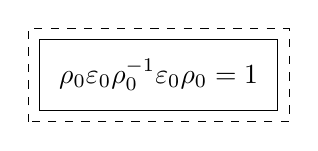
\begin{tikzpicture}\node[draw,inner sep=7pt] (r) {$\rho_0\varepsilon_0\rho_0^{-1}\varepsilon_0\rho_0=1$};\draw[dashed] ([xshift=-4pt,yshift=-4pt]r.south west) rectangle ([xshift=4pt,yshift=4pt]r.north east);\end{tikzpicture}}
Symétriques pour expression en $\varepsilon_1,\rho_1$ (relations $h_1$)
\margin{(à revoir!)}
\mspage{36}

\scanpage{38}
\mspage{3}
\textcircled{$\unsure{j_0|i_0}$}
\margin{$\varepsilon_0,\rho'_0$}
\[
\begin{gathered}
\varepsilon_1=\rho'_0(\varepsilon_0)=\rho'_0\varepsilon_0\rho_0'^{-1}\\
\sigma=\rho'_0\varepsilon_0^{-1}\\
\rho_0=\varepsilon_0\rho_0'^{-1}\varepsilon_0\\
\rho_1=\varepsilon_0^2\rho_0'^{-1}\\
\rho'_1=\varepsilon_0\rho'_0\varepsilon_0^{-1}
\end{gathered}
\qquad
\boxed{\begin{gathered}
\rho'_0=(\rho'_0(\varepsilon_0)\varepsilon_0)^2\\
\text{i.e.}\quad\rho'_0=(\rho'_0\varepsilon_0\rho_0'^{-1}\varepsilon_0)^2\\
\text{et}\quad[\rho_0'{}^3\deleted{\unsure{\varepsilon_0\rho'_0}},\varepsilon_0]=1
\end{gathered}}
\]
\uline{NB} On peut se borner à la seule équation abracadabrante:
\[
\unsure{\{}\rho'_0\underbrace{\varepsilon_0\rho_0'^{-1}\varepsilon_0\rho'_0}\varepsilon_0
\underbrace{\rho_0'^{-1}\varepsilon_0^{-1}\rho'_0\varepsilon_0^{-1}\rho_0'^{-1}}\varepsilon_0^{-1}=1
\]
\[
\text{i.e.}\quad[\rho'_0\underbrace{\varepsilon_0\rho_0'^{-1}\varepsilon_0\rho'_0},\varepsilon_0]=1
\]
qui implique
\diagram{\begin{tikzcd}[column sep=small]
\unsure{\varepsilon_0\rho_0'^{-1}\varepsilon_0\rho'_0}\arrow[d,bend right]&\deleted{\text{donc}}\ \rho'_0{}^{\deleted{\unsure{3}}}=(\rho'_0(\varepsilon_0)\varepsilon_0)^2\quad\text{donc}\\
(\unsure{-}\rho'_0(\varepsilon_0)\varepsilon_0)^3&
\end{tikzcd}}
Sym. pour expressions en $\varepsilon_1,\rho'_1$ (relations $(j_1)$)

\textcircled{$h'_0$}\deleted{$\unsure{j_0}$}
\margin{\figure{\begin{tikzpicture}\draw[->] (0,0) .. controls (-.2,1.8) and (-.3,4.8) .. (.4,5.6);\end{tikzpicture}}}
\margin{$\varepsilon_0,\rho_1$\par(\unsure{Ce cas se déduit de} $(h_0)$ par conjugaison par $\varepsilon_0$)\par\uline{NB} Il vaut mieux prendre $\uline{\varepsilon_1,\rho_0}$.}
\[
\begin{gathered}
\varepsilon_1=\rho_1^{-1}(\varepsilon_0)=\rho_1^{-1}\varepsilon_0\rho_1\\
\sigma=\rho_1^{-1}\varepsilon_0\\
\rho_0=\varepsilon_0^{-1}(\rho_1)=\varepsilon_0^{-1}\rho_1\varepsilon_0\\
\rho'_0=\deleted{\unsure{\rho_0}}=\varepsilon_0^{-1}(\rho_1^{-2})=\varepsilon_0^{-1}\rho_1^{-2}\varepsilon_0\\
\rho'_1=\rho_1^{-2}
\end{gathered}
\]
\figure{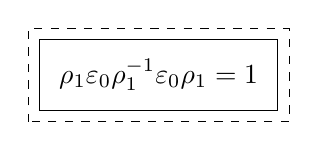
\begin{tikzpicture}\node[draw,inner sep=7pt] (r) {$\rho_1\varepsilon_0\rho_1^{-1}\varepsilon_0\rho_1=1$};\draw[dashed] ([xshift=-4pt,yshift=-4pt]r.south west) rectangle ([xshift=4pt,yshift=4pt]r.north east);\end{tikzpicture}}
Symétriques pour expressions en $(\varepsilon_1,\rho_0)$ (relations $h'_1$)

\textcircled{$j'_0$}
\margin{$\varepsilon_0,\rho'_1$}
\[
\begin{gathered}
\varepsilon_1=\rho_1'^{-1}(\varepsilon_0)=\rho_1'^{-1}\varepsilon_0\rho'_1\\
\sigma=\varepsilon_0^{-1}\rho'_1\\
\rho_1=\varepsilon_0\rho_1'^{-1}\varepsilon_0\\
\rho'_0=\varepsilon_0^{-1}(\rho'_1)=\varepsilon_0^{-1}\rho'_1\varepsilon_0\\
\rho_0=\rho_1'^{-1}\varepsilon_0^2
\end{gathered}
\qquad
\boxed{\begin{gathered}
\rho'_1=(\rho'_1(\varepsilon_0)\varepsilon_0)^2\\
\text{i.e.}\quad\rho'_1=(\rho'_1\varepsilon_0\rho_1'^{-1}\varepsilon_0)^2\\
\text{et}\quad[\rho_1'{}^3,\varepsilon_0]=1
\end{gathered}}
\]
Symétriques pour expressions en $(\varepsilon_1,\rho'_0)$ (relations \deleted{$\unsure{j_1}$} $\unsure{i'_0|j'_0}$)
\mspage{37}

\scanpage{39}
\mspage{4}
\uline{NB} Dans cette présentation, symétrie \unsure{s'exprime} par deux aut. involutifs de $H$
\diagram{$\begin{array}{l|ll}
1^\circ)\ g\longmapsto\check g&\varepsilon_0\longmapsto\varepsilon_0^{-1},&\varepsilon_1\longmapsto\varepsilon_1^{-1}\\
(\text{autom. }\uline{\text{ext.}})&\sigma\longmapsto\sigma^{-1}&\\
&\rho_0\longmapsto\rho_1^{-1},&\rho_1\longmapsto\rho_0^{-1}\\
&\rho'_0\longmapsto\rho_1'^{-1},&\rho'_1\longmapsto\rho_0'^{-1}
\end{array}$}
\diagram{$\begin{array}{l|ll}
2^\circ)\ g\longmapsto g^*&\varepsilon_0\longmapsto\varepsilon_1,&\varepsilon_1\longmapsto\varepsilon_0\\
&\sigma\longmapsto\sigma&\\
&\rho_0\longmapsto\rho_1,&\rho_1\longmapsto\rho_0\\
=\operatorname{int}(\sigma)&\rho'_0\longmapsto\rho'_1,&\rho'_1\longmapsto\rho'_0
\end{array}$}
\rule{25mm}{.4pt}

Ici symétrie centrée sur $\sigma$ ou $(\varepsilon_0,\varepsilon_1)$, symétrie binaire $(\sigma^2\in\operatorname{Cent}(H))$.
Si on centre la symétrie sur $\rho\mathrel{\mathop=^{\rm def}}\rho_0$, on trouve symétrie ternaire $(\rho^3\in\operatorname{Cent}(H))$, avec
\[
\varepsilon_0,\ \varepsilon_1=\rho(\varepsilon_0),\quad\varepsilon_\infty=\rho(\varepsilon_1)=\rho^2(\varepsilon_0)
\]
échangés circulairement par $\operatorname{int}(\rho)$,
\diagram{\begin{tikzcd}[column sep=large,row sep=large]
&\varepsilon_\infty\arrow[dl,dash,"\sigma_1=\varepsilon_\infty\varepsilon_0\varepsilon_\infty=\varepsilon_0\varepsilon_\infty\varepsilon_0"']\arrow[dr,dash,"\sigma_0=\varepsilon_1\varepsilon_\infty\varepsilon_1=\varepsilon_\infty\varepsilon_1\varepsilon_\infty"]&\\
\varepsilon_0\arrow[rr,dash,"\sigma_\infty=\varepsilon_0\varepsilon_1\varepsilon_0=\varepsilon_1\varepsilon_0\varepsilon_1"']&&\varepsilon_1
\end{tikzcd}}
\[\left(\begin{array}{c}\Vert\\\sigma\end{array}\right)\]
\[
\rho=(\varepsilon_1\varepsilon_0)^{-1}=(\varepsilon_\infty\varepsilon_1)^{-1}=(\varepsilon_0\varepsilon_\infty)^{-1}
\]
\deleted{$\unsure{\rho=\rho_0\quad(\rho_1)\quad\rho\rho\varepsilon\varepsilon}$}
\margin{\uline{NB} Mais les élémts\par
$\rho_1=(\varepsilon_0\varepsilon_1)^{-1}=\sigma_\infty(\rho)$\par
\deleted{$\unsure{\rho}$}$\ (\varepsilon_1\varepsilon_\infty)^{-1}=\sigma_0(\rho)=\rho(\rho_1)$\par
$(\varepsilon_\infty\varepsilon_0)^{-1}=\sigma_1(\rho)=\rho^2(\rho_1)$\par sont distincts}
\rule{28mm}{.4pt}

Les éléments essentiels du point de vue engendrement de $ST_{11}$ \deleted{sont} semblent être finalement
\[
\varepsilon_0,\varepsilon_1,\sigma,\rho\ (=\rho_0)
\]
plus l'élément
\[\omega=\rho^{-3}=\sigma^2\]
(qui engendre le centre)
\margin{\diagram{$\begin{array}{l}
(\varepsilon_0,\varepsilon_1)\\
(\varepsilon_0,\unsure{\sigma|\rho})\longleftrightarrow(\varepsilon_1,\sigma)\\
(\varepsilon_0,\rho)\longleftrightarrow(\varepsilon_1,\rho)\\
(\sigma,\rho)
\end{array}$}
\unsure{Les quatre expressions de syst. de gén. principaux} de $ST_{11}$.}
\mspage{38}

\scanpage{40}
\mspage{5}
\margin{(1983)}
\textcircled{1} $(\varepsilon_0,\varepsilon_1)$,\quad
$\boxed{\boxed{\varepsilon_0\varepsilon_1\varepsilon_0=\varepsilon_1\varepsilon_0\varepsilon_1}}$
\[
\left\{\begin{aligned}
\sigma&=\varepsilon_0\varepsilon_1\varepsilon_0=\varepsilon_1\varepsilon_0\varepsilon_1\\
\rho&=(\varepsilon_1\varepsilon_0)^{-1}
\end{aligned}\right.
\]
\textcircled{2} $(\varepsilon_0,\sigma)$,\quad
$\boxed{[\sigma^2,\varepsilon_0]=1,\quad(\sigma^{-1}\varepsilon_0)^{-3}=\sigma^2}$
\[
\left\{\begin{aligned}
\varepsilon_1&=\sigma(\varepsilon_0)=\sigma\varepsilon_0\sigma^{-1}\\
\rho&=\sigma^{-1}\varepsilon_0
\end{aligned}\right.
\]
\margin{[\uline{sym}\quad$\begin{gathered}\varepsilon_0=\sigma(\varepsilon_1)=\sigma\varepsilon_1\sigma^{-1}\\\rho=\varepsilon_1\sigma^{-1}\end{gathered}$]}
\textcircled{3} $(\varepsilon_0,\rho)$\quad
$\boxed{\boxed{\rho\varepsilon_0\rho^{-1}\varepsilon_0\rho=1}}$
\[
\left\{\begin{aligned}
\varepsilon_1&=\rho(\varepsilon_0)=\rho\varepsilon_0\rho^{-1}\\
\sigma&=\varepsilon_0\unsure{\rho_0^{-1}|\rho^{-1}}
\end{aligned}\right.
\]
\margin{[sym\quad$\begin{gathered}\varepsilon_0=\rho^{-1}(\varepsilon_1)=\rho^{-1}\varepsilon_1\rho\\\sigma=\rho^{-1}\varepsilon_1\end{gathered}$]}
\textcircled{4} $(\sigma,\rho)$\quad$\boxed{\boxed{\rho^{-3}=\sigma^2}}$
\[
\left\{\begin{aligned}\varepsilon_0&=\sigma\rho\\\varepsilon_1&=\rho\sigma\end{aligned}\right.
\]
\rule{\linewidth}{.4pt}\par\rule{\linewidth}{.4pt}
\diagram{$\begin{array}{l|ll|l}
\varepsilon_0,\varepsilon_1,\sigma,\rho\ \deleted{\unsure{\rho_0}}&\varepsilon_0=\sigma\rho&\sigma=\varepsilon_0\varepsilon_1\varepsilon_0=\varepsilon_1\varepsilon_0\varepsilon_1&\boxed{\varepsilon_0\varepsilon_1\varepsilon_0=\varepsilon_1\varepsilon_0\varepsilon_1}\\
&\varepsilon_1=\rho\sigma&\rho=(\varepsilon_1\varepsilon_0)^{-1}=\varepsilon_0^{-1}\varepsilon_1^{-1}&\boxed{\begin{gathered}\rho^{-3}=\sigma^2\ (\mathrel{\mathop=^{\rm def}}\omega)\\\uline{\text{central}}\end{gathered}}\\
&\multicolumn{2}{l|}{\sigma(\varepsilon_0)=\rho(\varepsilon_0)=\varepsilon_1}&\boxed{\rho\varepsilon_0\rho^{-1}\varepsilon_0\rho=1}\\
&\multicolumn{2}{l|}{\sigma(\varepsilon_1)=\rho^{-1}(\varepsilon_1)=\varepsilon_0}&\\\cline{2-4}
\end{array}$}

Pour un formulaire plus complet, il faudrait

a) Introduire aussi $\varepsilon_\infty$, \deleted{\unsure{les}} les $\ell_i=\varepsilon_i^2$ $(i\in\{0,1,\infty\})$.

b) Introduire aussi les $\tau_i$ $(i\in\{0,1,\infty\})$ pour $ST_{11}^{\unsure{\pm}}$.

c) Donner (par la relation suppl. $\omega^2=1$) la représentation matricielle dans $GL(2,\mathbb Z)$.
\mspage{39}

\scanpage{42}
\mspage{1}
\diagram{\begin{tikzcd}[column sep=huge,row sep=large]
\deleted{\unsure{an}}\ PM_{1,1}\arrow[d]&P\mathcal D\simeq\{z_1,z_2\in\mathbb C\mid z_1/\deleted{\unsure{z_1}}\inserted{z_2}\in\mathcal D\}\simeq\operatorname{Hom}^{\unsure{+|*}}(\mathbb Z^2,\mathbb C)\arrow[l]\arrow[d,"{(z_1,z_2)\longmapsto z_2/z_1}"]\\
M_{1,1}&\begin{gathered}\mathcal D\simeq\widetilde M_{1,1}\\\Vert\\\{z\in\mathbb C\mid\operatorname{Im}z>0\}\end{gathered}\arrow[ul,phantom,"\text{cart}" description]\arrow[l,"{\text{gal. groupe }SL(2,\mathbb Z)}"']
\end{tikzcd}}
\deleted{$\unsure{\text{et }z_1/z_2\quad\mathcal D\times\mathbb C^*}$}
(rigidification de Torelli stricte, i.e. avec $\varphi(e_1,e_2)=+1$, $e_2/e_1=\tau\in\mathcal D$)
\figure{\begin{tikzpicture}[scale=1.1]\draw[->,thick] (0,0)--(-.3,1.7) node[above]{$\unsure{z_2}$};\draw[->,thick] (0,0)--(.9,.8) node[right]{$\unsure{z_1}$};\draw[->] (2,.35) .. controls (2.5,.9) and (2.2,1.2) .. (1.9,1.05);\end{tikzpicture}}
\figure{\begin{tikzpicture}\draw[->] (0,0)--(2.4,0);\node[above] at (1.3,0){$\mathbb Z^2$};\node at (.15,0){\deleted{$\unsure{e_\infty}$}};\end{tikzpicture}}
\[
\begin{pmatrix}a&b\\c&d\end{pmatrix}\begin{pmatrix}x\\y\end{pmatrix}=\begin{pmatrix}ax+by\\cx+dy\end{pmatrix}
\]
\[
\begin{pmatrix}a&b\\c&d\end{pmatrix}(z)=\deleted{\frac{dz+c}{bz+a}}\ \frac{az+b}{cz+d}
\]
$\mathbb C^*\times SL(2,\mathbb Z)$ opère sur $P\mathcal D$ par
\[(z_1,z_2)\longmapsto\lambda(az_1+bz_2,cz_1+dz_2).\]
\unsure{Alors} par passage au quotient, $SL(2,\mathbb Z)$ opère sur $P\mathcal D/\mathbb C^*\simeq\mathcal D$.
C'est induit par l'opération naturelle de $GL(2,\mathbb R)$ sur $\widehat{\mathbb C}=\mathbb P^1(\mathbb C)$
\[
\begin{pmatrix}a&b\\c&d\end{pmatrix}(z)=\frac{az+b}{cz+d}
\]
\diagram{$\begin{array}{c}SL(2,\mathbb R)\\\cup\\SL(2,\mathbb Z)\end{array}$}
invarie $\mathcal D$\quad(i.e. $SL(2,\mathbb R)\simeq\operatorname{Aut}_{\mathbb C}(\mathcal D)$)
\[
\boxed{\begin{gathered}
M_{1,1}^{an}\deleted{(\mathbb C)}\simeq(\mathcal D,SL(2,\mathbb Z))\\
PM_{1,1}^{an}\deleted{(\mathbb C)}\simeq(P\mathcal D,SL(2,\mathbb Z))
\end{gathered}}
\]
\margin{$M_{11}^{\unsure{conf}}\deleted{(\mathbb C)}\simeq(\mathcal D,GL(2,\mathbb Z))$\par
$PM_{11}^{\unsure{conf}}\simeq(P\mathcal D,GL(2,\mathbb Z))$}
\[
\mathcal T_{11}\simeq SL(2,\mathbb Z)\qquad S\mathcal T_{11}\simeq\widetilde{SL}(2,\mathbb Z)
\]
\margin{$GL^{\pm1}(2,\mathbb R)$ opère sur $P\mathcal D$ par\par
$(z_1,z_2)\longrightarrow(a\tau^\alpha z_1+b\tau^\alpha z_2,c\tau^\alpha z_1+d\tau^\alpha z_2)$\par
\deleted{$\unsure{g}$}$\ u_g=\tau^{\alpha(g)}\cdot g$\par
$\left\{\begin{gathered}\alpha(g)\in\mathbb Z/2\mathbb Z\\\alpha(g)=0\quad\text{si }\det g=1\\=1\quad\text{si }\det g=-1\end{gathered}\right.$}
\mspage{41}

\scanpage{43}
\mspage{2}
Section $\tau\longmapsto(\tau,1)$ de $P\mathcal D$ sur $\mathcal D$, d'où iso
\deleted{$P\mathcal D\simeq\mathcal D$}
\diagram{\begin{tikzcd}[column sep=large]
\mathcal D\times\mathbb C^*\arrow[r]&P\mathcal D\\
(\tau,\lambda)\arrow[r,mapsto]&\lambda(\tau,1)=(\lambda\tau,\lambda)\mathrel{\mathop=^{\rm def}}[\tau,\lambda]
\end{tikzcd}}
on trouve
\[
\left\{\begin{gathered}
\lambda'[\tau,\lambda]=[\tau,\lambda'\lambda]\\
\begin{pmatrix}a&b\\c&d\end{pmatrix}([\tau,\lambda])=\left[\frac{a\tau+b}{c\tau+d},\lambda(c\tau+d)\right]
\end{gathered}\right.
\]
\diagram{\begin{tikzcd}[column sep=large]
\widetilde{PM}_{11}^{an}\simeq\mathcal D\times\mathbb C\arrow[r]&P\mathcal D\\
(\tau,z)\arrow[r,mapsto]&(\exp 2\pi iz)(\tau,1)=[\tau,\exp 2i\pi z]
\end{tikzcd}}
\[
\begin{array}{c}\omega^2\\\unsure{\ni}\\\mathbb Z\end{array}\subset\widetilde{SL}(2,\mathbb Z)\quad\deleted{\unsure{\text{aut}}}
\]
opère sur $\mathcal D\times\mathbb C$ de façon compatible avec l'action sur $P\mathcal D$ et $\omega^2\in\mathbb Z$ opérant par
\[(\tau,\unsure{\tau|z})\longmapsto(\tau,z+1)\]
\rule{\linewidth}{.4pt}

Pts fixes de $z\longmapsto\dfrac{az+b}{cz+d}$ donnés par
\[cz^2+(d-a)z-b=0\]
\margin{$\Delta=(d-a)^2+4bc=(a+d)^2-4$\par car $bc=ad-1$}
Ici $a,b,c,d\in\mathbb Z\subset\mathbb R$, --- \unsure{on s'intéresse} \deleted{$\Delta\Leftarrow$} au cas où $\exists z$ pt fixe $\in\mathcal D$ i.e. $z\notin\mathbb R$ i.e.

GP

THEMATIQUE.

\unsure{on a}\quad$\Delta<0$ i.e. $|a+d|\leq1$

Deux cas\quad\deleted{$a+d$}
\[
1^\circ)\quad a+d=0\qquad d=-a\qquad z\longrightarrow\frac{az+b}{cz-a}
\]
\[d-a=-2a\]
\margin{$-a^2-bc=1$\par$bc=-1-a^2$}
\[
cz^2-2az-b=0\qquad z=\frac{a\pm2i}{2c}
\]
On trouve \textcircled{$\unsure{\mathbb Z/4|4}$}

pour $a=0$, \deleted{$\unsure{d=-1}$} $d=0$, $b=\deleted{\unsure{0}}-1$, $c=1$, $z=i$.
\mspage{42}

\scanpage{44}
MINISTÈRE\par DE L'ÉDUCATION\par\rule{9mm}{.4pt}

Délégation aux Relations\par Universitaires Internationales\par --\par\rule{10mm}{.4pt}

Bureau Amérique Latine,\par Afrique, Pays Arabes,\par Asie du Sud Est.

PARIS, LE\quad 15 FEV. 1982

LE MINISTRE DE L'EDUCATION NATIONALE

A Mesdames et Messieurs

- Les Recteurs Chanceliers\par
- Les Directeurs et Présidents\par des Grands Etablissements\par
- Les Présidents d'Universités\par et des Centres Universitaires\par
- Les Présidents d'Instituts Nationaux\par Polytechniques et les Directeurs des\par Ecoles d'Ingénieurs Indépendantes des\par Universités\par
- Les Directeurs des E.N.S.I.\par
- Les Directeurs des I.U.T.

\figure{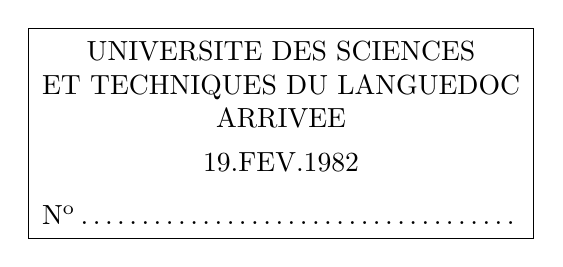
\begin{tikzpicture}\node[draw,align=center,inner sep=5pt] {\unsure{UNIVERSITE DES SCIENCES}\\\unsure{ET TECHNIQUES DU LANGUEDOC}\\\unsure{ARRIVEE}\\[4pt]19.FEV.1982\\[7pt]N\textsuperscript{o}\dotfill};\end{tikzpicture}}
\unsure{N\textsuperscript{o}}\quad 0153

\uline{OBJET} : Recrutement d'enseignants en coopération.

Le Ministère des Relations Extérieures vient de me faire tenir l'état des besoins en personnels enseignants dans les universités maghrébines pour l'année 1982 - 1983.

Je vous serais très obligé de bien vouloir procéder à la diffusion la plus large possible de cette liste dans votre établissement.

En effet, les premières sessions des Commissions Mixtes de recrutement pour les trois pays du Maghreb, doivent se tenir sous peu.

Il serait souhaitable d'inviter les candidats enseignants titulaires d'un grade de l'enseignement supérieur et les candidats non titulaires à adresser, directement et dans les meilleurs délais, leur demande accompagnée de leur curriculum vitae au C.F.E.C.T.I. \unsure{Carrefcur|Carrefour} coopération - 34, rue Dumont Durville 75016 PARIS.

En ce qui concerne les professeurs agrégés du second degré ou les titulaires de l'enseignement technique, ils devront transmettre d'urgence leur candidature et leur curriculum vitae au Ministère de l'Education Nationale - Direction des Personnels Enseignants de Lycées - Service de la réglementation et de la gestion - sous direction de la gestion des personnels enseignants - Bureau D P E 9 - 34, rue de Châteaudun - 75009 PARIS.

\figure{\begin{tikzpicture}\draw[thick] (0,0)--(8,0);\draw[thick] (7.65,.2)--(9.5,-2.8);\end{tikzpicture}}
DIFFUSION : LISTE C n\textsuperscript{o} 1049, NC.PB

Transmis par la Cellule des Relations Internationales (bâtiment administratif, niveau haut) où vous pourrez consulter la liste des postes par disciplines et grades

MONTPELLIER, le 23 Février 1982

Le Délégué aux Relations\par Internationales

\figure{
\begin{tikzpicture}[scale=.65]\draw (0,0)--(.45,1.4)--(.65,-.15) (.03,.3)--(.8,.7);\draw (.6,.1) .. controls (1.1,1.7) and (1.7,1.8) .. (.9,.5) .. controls (1.2,.5) and (1.4,1.4) .. (1.55,1.25) .. controls (1.3,.8) and (1.1,.2) .. (1.5,.4) .. controls (1.65,.8) and (1.65,1.05) .. (1.75,.4) .. controls (1.75,.2) and (1.95,.9) .. (2.1,.75) .. controls (2.4,.6) and (2.6,1.2) .. (2.8,.8) .. controls (3,.8) and (2.5,.1) .. (2.75,.2);\draw (0,-.1)--(3.6,1);\end{tikzpicture}}
A. PAVIA

L'Adjoint au Délégué\par chargé des Affaires Administratives\par et Financières

\figure{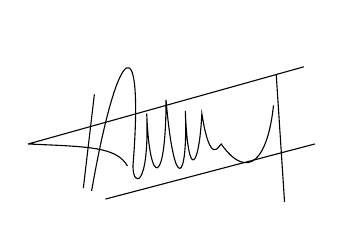
\begin{tikzpicture}[scale=.7]\draw (0,.9)--(5,2.3) (0,.9) .. controls (1.1,.85) and (1.6,.85) .. (1.8,.5);\draw (1,.1)--(1.2,1.8) (1.15,.05) .. controls (1.65,2.9) and (2.1,3) .. (1.9,.5) .. controls (1.9,.1) and (2.2,.1) .. (2.15,1.45) .. controls (2.2,.1) and (2.5,.1) .. (2.5,1.7) .. controls (2.65,-.05) and (2.9,.2) .. (2.85,1.5) .. controls (2.9,.2) and (3.1,.45) .. (3.15,1.45) .. controls (3.3,.5) and (3.45,.85) .. (3.5,.9) .. controls (4,.2) and (4.35,.65) .. (4.45,1.6);\draw (4.5,2.15)--(4.65,-.15) (1.4,-.1)--(5.2,.9);\end{tikzpicture}}
Jean Louis DEVAUX
\mspage{43}

\scanpage{45}
\mspage{3}
\[
2^\circ)\quad a+d=1\quad\text{i.e.}\quad d=1-a
\]
p.ex. $a=0$, $d=1$, $bc=-1$\qquad$b=1,c=-1$
\[
\rho=\begin{pmatrix}0&1\\-1&1\end{pmatrix},\qquad
z=\frac12+i\frac{\sqrt3}{2}=\exp\frac{2i\pi}{6}=\unsure{\jmath|\zeta}
\]

MR\quad COUPIAC LOUIS-BERNARD

ALLOCATAIRE DE RECHERCHES

\margin{R}

U.E.R. DE MATHEMATIQUES
\mspage{44}

\scanpage{46}
MINISTÈRE\par DE L'ÉDUCATION\par\rule{9mm}{.4pt}

Délégation aux Relations\par Universitaires Internationales\par --\par\rule{10mm}{.4pt}

Bureau Amérique Latine,\par Afrique, Pays Arabes,\par Asie du Sud Est.

PARIS, LE\quad 15 FEV. 1982

LE MINISTRE DE L'EDUCATION NATIONALE

A Mesdames et Messieurs

- Les Recteurs Chanceliers\par
- Les Directeurs et Présidents\par des Grands Etablissements\par
- Les Présidents d'Universités\par et des Centres Universitaires\par
- Les Présidents d'Instituts Nationaux\par Polytechniques et les Directeurs des\par Ecoles d'Ingénieurs Indépendantes des\par Universités\par
- Les Directeurs des E.N.S.I.\par
- Les Directeurs des I.U.T.

\figure{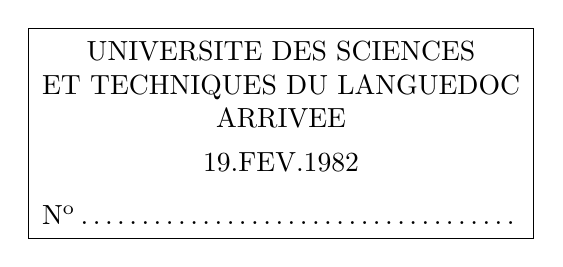
\begin{tikzpicture}\node[draw,align=center,inner sep=5pt] {\unsure{UNIVERSITE DES SCIENCES}\\\unsure{ET TECHNIQUES DU LANGUEDOC}\\\unsure{ARRIVEE}\\[4pt]19.FEV.1982\\[7pt]N\textsuperscript{o}\dotfill};\end{tikzpicture}}
\unsure{N\textsuperscript{o}}\quad 0153

\uline{OBJET} : Recrutement d'enseignants en coopération.

Le Ministère des Relations Extérieures vient de me faire tenir l'état des besoins en personnels enseignants dans les universités maghrébines pour l'année 1982 - 1983.

Je vous serais très obligé de bien vouloir procéder à la diffusion la plus large possible de cette liste dans votre établissement.

En effet, les premières sessions des Commissions Mixtes de recrutement pour les trois pays du Maghreb, doivent se tenir sous peu.

Il serait souhaitable d'inviter les candidats enseignants titulaires d'un grade de l'enseignement supérieur et les candidats non titulaires à adresser, directement et dans les meilleurs délais, leur demande accompagnée de leur curriculum vitae au C.F.E.C.T.I. \unsure{Carrefcur|Carrefour} coopération - 34, rue Dumont Durville 75016 PARIS.

En ce qui concerne les professeurs agrégés du second degré ou les titulaires de l'enseignement technique, ils devront transmettre d'urgence leur candidature et leur curriculum vitae au Ministère de l'Education Nationale - Direction des Personnels Enseignants de Lycées - Service de la réglementation et de la gestion - sous direction de la gestion des personnels enseignants - Bureau D P E 9 - 34, rue de Châteaudun - 75009 PARIS.

\figure{\begin{tikzpicture}\draw[thick] (0,0)--(8,0);\draw[thick] (7.65,.2)--(9.5,-2.8);\end{tikzpicture}}
DIFFUSION : LISTE C n\textsuperscript{o} 1049, NC.PB

Transmis par la Cellule des Relations Internationales (bâtiment administratif, niveau haut) où vous pourrez consulter la liste des postes par disciplines et grades

MONTPELLIER, le 23 Février 1982

Le Délégué aux Relations\par Internationales

\figure{
\begin{tikzpicture}[scale=.65]\draw (0,0)--(.45,1.4)--(.65,-.15) (.03,.3)--(.8,.7);\draw (.6,.1) .. controls (1.1,1.7) and (1.7,1.8) .. (.9,.5) .. controls (1.2,.5) and (1.4,1.4) .. (1.55,1.25) .. controls (1.3,.8) and (1.1,.2) .. (1.5,.4) .. controls (1.65,.8) and (1.65,1.05) .. (1.75,.4) .. controls (1.75,.2) and (1.95,.9) .. (2.1,.75) .. controls (2.4,.6) and (2.6,1.2) .. (2.8,.8) .. controls (3,.8) and (2.5,.1) .. (2.75,.2);\draw (0,-.1)--(3.6,1);\end{tikzpicture}}
A. PAVIA

L'Adjoint au Délégué\par chargé des Affaires Administratives\par et Financières

\figure{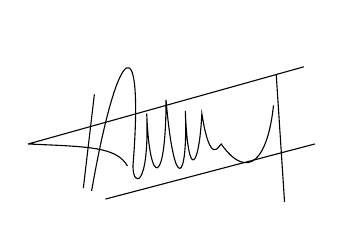
\begin{tikzpicture}[scale=.7]\draw (0,.9)--(5,2.3) (0,.9) .. controls (1.1,.85) and (1.6,.85) .. (1.8,.5);\draw (1,.1)--(1.2,1.8) (1.15,.05) .. controls (1.65,2.9) and (2.1,3) .. (1.9,.5) .. controls (1.9,.1) and (2.2,.1) .. (2.15,1.45) .. controls (2.2,.1) and (2.5,.1) .. (2.5,1.7) .. controls (2.65,-.05) and (2.9,.2) .. (2.85,1.5) .. controls (2.9,.2) and (3.1,.45) .. (3.15,1.45) .. controls (3.3,.5) and (3.45,.85) .. (3.5,.9) .. controls (4,.2) and (4.35,.65) .. (4.45,1.6);\draw (4.5,2.15)--(4.65,-.15) (1.4,-.1)--(5.2,.9);\end{tikzpicture}}
Jean Louis DEVAUX
\mspage{45}

\scanpage{47}
\mspage{4}
\figure{\begin{tikzpicture}[scale=1.4]
\draw (-2.1,0)--(2.2,-.03);\draw (-1,0) arc[start angle=180,end angle=0,radius=1];\draw (0,-1)--(0,3.35);\draw (.5,0)--(.5,3.35);
\draw[thick] (0,1)--(0,3.35) (.5,.866)--(.5,3.35);
\draw (0,1.15)--(.5,1.55) (0,1.7)--(.5,2.1) (0,2.25)--(.5,2.65) (0,2.8)--(.5,3.2) (0,3.15)--(.22,3.35);
\fill (0,1) circle(.025) (.5,.866) circle(.025);\node[left] at (0,1.12){$\uline{i}$};\node[right] at (.5,.866){$\jmath$};
\end{tikzpicture}}
\[
\rho=\deleted{\unsure{\sigma}}\begin{pmatrix}0&1\\-1&1\end{pmatrix}\qquad\rho^3=\omega=\begin{pmatrix}-1&0\\0&-1\end{pmatrix}
\]
\[
\sigma=\begin{pmatrix}0&+1\\-1&0\end{pmatrix}\qquad\sigma^2=\omega\qquad\sigma^{-1}=\omega\sigma
\]
On a choisi les signes de telle façon pour

a) $\rho^3=\deleted{\unsure{1}}-1$ i.e. $\rho$ d'ordre $6$ i.e. il engendre le groupe d'isotropie \inserted{de $\jmath$} (mais cela laisse le choix entre $\rho$ et $\rho^{-1}$)

b) $\sigma$ soit la rotation de l'angle $-\dfrac\pi2$ dans $\mathbb R^2$ (pour la structure euclidienne habituelle) et que $\rho$ soit une rotation d'angle $-2\pi/6$ (pour une métrique invariante convenable).
La chose importante dans cette convention, \unsure{c'est} que pour $\rho$ et $\sigma$, le sens des rotations (i.e. négatif) soit le $\unsure{\overline{\mathrm m}}$.
Quand on interprète \deleted{que} les matrices $\begin{pmatrix}a&b\\c&d\end{pmatrix}\in SL(2,\mathbb Z)$ comme opérant sur des \deleted{\unsure{systèmes}}\inserted{couples} $(z_1,z_2)$ de vecteurs de $\mathbb C$, engendrant un sous-groupe discret de $\mathbb C$ (avec $z_1/z_2\in\mathcal D$), alors l'action de $\rho$ et de $\sigma$ sur $z_1,z_2$ est ``positive'', en ce sens que $(z_1,u(z_1))$ et $(z_2,u(z_2))$ forment des $\mathbb R$-bases \uline{directes} de $\mathbb C\simeq\mathbb R^2$.

Voyons le groupe des relèvements de $SL(2,\mathbb Z)$ opérant sur $P\mathcal D$ sur $\widetilde{P\mathcal D}$, qui est donc une extension centrale de $\mathcal T_{11}=\unsure{GL|SL}(2,\mathbb Z)$ par $\mathbb Z$, \deleted{\unsure{soit}}\inserted{qui peut s'écrire $S\mathcal T_{11}$}\deleted{$\widetilde{SL}(2,\mathbb Z)$}.
Je désigne par \deleted{$\unsure{\omega}$} $\overline\omega$ l'élément de \deleted{$SL(2,\mathbb Z)$} $S\mathcal T_{11}$ défini par le générateur de $\mathbb Z$, opérant sur $\widetilde{P\mathcal D}$ par $(\tau,z)\mathrel{\text{---}}(\tau,z+1)$.
\mspage{46}

\scanpage{48}
\deleted{
\begin{center}
UNIVERSITÉ DES SCIENCES\\
ET TECHNIQUES DU LANGUEDOC\\\rule{17mm}{.3pt}
\end{center}
\hfill Montpellier, le

\begin{center}
\uline{A N N E X E\quad I}\textsuperscript{(1)}

\uline{RENSEIGNEMENTS A FOURNIR PAR LE DIRECTEUR DE RECHERCHE}
\end{center}

\uline{NOM et Prénom du Candidat} : \rule{7cm}{0.3pt}

\uline{Titre de la thèse} : \rule{9cm}{0.3pt}

\noindent\rule{13cm}{0.3pt}\\
\rule{13cm}{0.3pt}

\uline{NOM du Directeur de thèse} : \rule{8cm}{0.3pt}

\uline{Désignation du laboratoire où la thèse est préparée} : \rule{5cm}{0.3pt}

\noindent\rule{13cm}{0.3pt}

\uline{Durée approximative des recherches ayant abouti à la thèse} : \rule{4cm}{0.3pt}

\uline{Rapporteurs proposés}\textsuperscript{(1)} :
\diagram{$\begin{array}{rllll}
&\text{NOM et Prénom}&\text{Titre}&\text{Spécialité}&\begin{array}{c}\text{Etablissement, Université, où sont}\\\text{exercées les fonctions}\end{array}\\[1ex]
1\;{-}&\multicolumn{4}{l}{\rule{11cm}{0.3pt}}\\[1ex]
2\;{-}&\multicolumn{4}{l}{\rule{11cm}{0.3pt}}\\[1ex]
3\;{-}&\multicolumn{4}{l}{\rule{11cm}{0.3pt}}
\end{array}$}

\textit{Signature du Candidat,}\hfill\textit{Signature du Directeur de Recherche,}

\uline{Avis du Président} : \rule{10cm}{0.3pt}

\noindent\rule{3cm}{0.6pt}

(1) Une au moins de ces personnalités doit ne pas appartenir au corps enseignant de l'Université des Sciences et Techniques du Languedoc.\\
L'un d'eux doit être le Directeur de Recherche du candidat.\\
Les rapporteurs ont un délai de 15 jours pour établir le rapport.\\
Le candidat ne pourra soutenir qu'au minimum 3 semaines après la date de réception de ces rapports.
}
\mspage{47}

\scanpage{49}
\hfill\uline{2-\unsure{cartes} \unsure{cellulaires}}

\mspage{48}

\scanpage{50}
\hfill\begin{tabular}{c}\uline{\unsure{Manipulations} sur les cartes}\\\uline{cellulaires}\end{tabular}

\[
(X,G)=\Pi_1(X,G)
\]
\[
\operatorname{Hom}_{(X,G)}(x,y)=\{(\ell,g)\mid
\underbrace{\ell:gx\longrightarrow y}_{\in\,\unsure{\mathrm{Fl}|\mathrm{FC}}\,\Pi_1X},\quad g\in G\}
\]
\diagram{\begin{tikzcd}[column sep=small,row sep=small]
gx\arrow[r,"\ell"]&y&\\
&g'y\arrow[r,"\ell'"]&z
\end{tikzcd}}
\[
\boxed{(\ell',g')(\ell,g)=(\ell'\circ g'(\ell),g'g)}
\]

\mspage{49}

\scanpage{51}
1. Description combinatoire des cartes, via $G_2$ et $G_2^\circ$\hfill p. 1

2. Cartes tri-angulaires pondérées, et groupes $\Pi_{03}$, $\Pi_{0,3}^\tau$\hfill p. 4.

3. Relation aux revêtements de $U_{0,3}$ et courbes algébriques\hfill p. $5'$

4. Conditions $\unsure{\rho_i|\beta_i}^{\nu_i}=1$ et groupes fondamentaux à signature\hfill p. $9'$

5. Sur l'existence d'une pondération d'une carte tri-angulaire\hfill p. $12'$

6. Carte associée à un polygône courbe, et groupes fondamentaux associés\hfill p. 15

7. Relation aux cartes $n$-polygonales pondérées\hfill p. 22.

8. Introduction de $P\Sigma^*_{\unsure{P_n|\rho_n}}$ et du 2-groupoïde fondamental\hfill p. 29

\mspage{50}

\scanpage{52}
\mspage{1}

Rétrospection sur les cartes. (finies)

\textcircled{1} Définition initiale \inserted{d'une \uline{carte} (topologique) cellulaire}: surface compacte (pas néc. orientable) $X$, avec partie fermée $K$, loc. \unsure{homéom.} à une étoile (``1-complexe topologique''), plus hypothèses ``cellulaires'': a) $K$ n'a pas de composantes connexes homéom. à $S^1$ \deleted{\unsure{ni de}} \inserted{ni de points isolés} b) Les comp. connexes de $X-K$ sont des disques ouverts i.e. homéom. à $\mathring D=\{z\in\mathbb C\mid |z|<1\}$.

\margin{b) implique déjà que $K$ n'a pas de pt isolé, \uline{sauf} \deleted{\unsure{quand}} il y a une comp. connexe $X_0$ de $X$ \deleted{\unsure{réduite qui}} est une sphère, avec $K\cap X_0$ réduit à un point.}

On en fait une ``catégorie isotopique'', et à l'aide de la notion de \unsure{biarc} (p.ex.), on établit une équivalence de catégories
\[
(1)\qquad \deleted{\text{\unsure{Cartes}}}\quad\text{Cartes isot.}\ \underset{\rule{1.1cm}{0.3pt}}{\approx}\ G_2\text{-ensembles }\inserted{\text{finis}}\text{ ``spéciaux''}
\]
où
\[
(2)\qquad G_2\simeq\{\tau_0,\tau_1,\underbrace{\tau_2}_{\text{ou }\tau_\infty}\mid
\tau_0^2=\tau_1^2=\tau_2^2=(\tau_0\tau_2)^2=1\}
\]
(\uline{NB} Par la suite, on notera $\unsure{\sigma_\infty|\tau_\infty}$ en lieu de $\unsure{\sigma_2|\tau_2}$, notation mieux appropriée pour les relations avec les Cour. Alg. La notation $\unsure{\sigma_2|\tau_2}$ est plus appropriée pour les généralisations en dim supérieure $\ldots$),
\margin{La notation $\unsure{\sigma_2|\tau_2}$ est plus commode p.ce. qu'on dira que $\unsure{\sigma_i|\tau_i}$ est l'opération (sur les repères) qui \unsure{change le $i$-feuillet du repère en le} \unsure{de façon à fixer les autres}.}
et où les $G$-ens ``spéciaux'' sont ceux où les involutions
\[
\tau_0,\tau_1,\tau_2\quad\text{et}\quad\sigma=\tau_0\tau_2
\]
opèrent sans points fixes. (NB. Par la suite, on pose $\rho_1=\tau_0\tau_\infty$, en $=$ temps qu'on écrit $\tau_\infty$ pour $\tau_2$.)

On introduit
\[
(3)\qquad G_2^\circ=\operatorname{Ker}\left(\begin{array}{rcl}
G_2&\longrightarrow&\mathbb Z/2\mathbb Z\\
\tau_i&\longmapsto&1\bmod2
\end{array}\right)
\]
et on a
\[
\unsure{(4)}\qquad G_2^\circ=\{\rho_0,\rho_1,\rho_\infty\mid\rho_\infty\rho_1\rho_0=\deleted{\unsure{1}}\rho_1^2=1\}
\]
\mspage{51}

\scanpage{53}
avec
\[
(5)\qquad\rho_\infty=\tau_1\tau_0,\quad\rho_1=\tau_0\tau_\infty,\quad\rho_0=\tau_\infty\tau_1
\]

La relation avec les ``repères'', en tant que simplexes topologiques de la subdivision barycentrique, est la suivante:

\figure{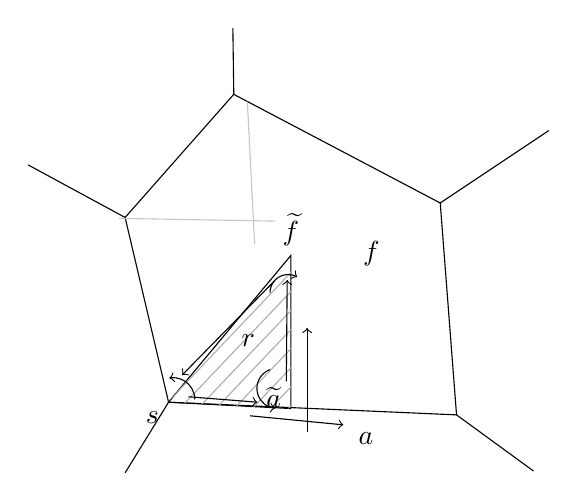
\begin{tikzpicture}[scale=1.15]
\coordinate (s) at (0,0);\coordinate (aa) at (1.35,-.07);\coordinate (ff) at (1.35,1.62);
\draw (s)--(-.48,2.04)--(.72,3.4)--(3,2.2)--(3.18,-.14)--cycle;
\draw (s)--(-.48,-.78) (-.48,2.04)--(-1.55,2.62) (.72,3.4)--(.71,4.13) (3,2.2)--(4.2,3) (3.18,-.14)--(4.03,-.76);
\draw[gray!45,thin] (-.55,2.03)--(1.18,2) (.87,3.32)--(.95,1.75);
\draw (s)--(ff)--(aa)--cycle;
\begin{scope}\clip (s)--(ff)--(aa)--cycle;
\foreach \x in {-1,-.8,...,1.3}{\draw[gray!65,thin] (\x,-.2)--(\x+1.9,1.8);}\end{scope}
\draw[->] (.22,.06)--(.98,0);
\draw[->] (1.3,.23)--(1.31,1.35);
\draw[->] (1.17,1.34)--(.15,.3);
\draw[->] (.29,.03) arc (0:100:.24);
\draw[->] (1.12,.36) arc (110:265:.22);
\draw[->] (1.12,1.21) arc (180:60:.2);
\draw[->] (1.53,-.33)--(1.53,.82);
\draw[->] (.9,-.15)--(1.93,-.25);
\node[below left] at (s) {$s$};\node[left] at (1.35,.05) {$\widetilde a$};
\node[above] at (ff) {$\widetilde f$};\node at (.88,.68) {$r$};\node at (2.24,1.64) {$f$};\node[below] at (2.18,-.23) {$a$};
\end{tikzpicture}}

Le biarc \inserted{associé au repère $r$} a comme orientation tangentielle celle qui \uline{sort} du sommet $s$, comme orientation normale celle qui \uline{entre} dans la face $f$ (``on sort des sommets pour entrer dans la face $f$, en passant par l'arête $a$''). Les trois sommets de $r$ sont le sommet $s=\widetilde s$, le ``centre'' $\widetilde a$ de $a$, et le ``centre'' $\widetilde f$ de $f$, l'orientation de $r$ est celle qui tourne autour de $r$ dans le sens $s\,\widetilde a\,\widetilde f$ (comme le dit la \unsure{notation} image plus bas).

C'est aussi celle pour laquelle l'\deleted{\unsure{flèche}} orientation normale \inserted{de l'arête $a$} indique le sens de rotation direct autour du sommet $s$, \inserted{``origine'' de $a$ pour l'orientation tangentielle choisie)}, et pour laquelle l'orientation tangentielle indique le sens de rotation autour de $f$ (``\unsure{fin extrémité}'' de $a$, pour l'orientation normale du biarc). Les sens de rotation ``directe'' (pour l'orientation définie par $r$) autour des trois sommets de $r$ sont indiqués sur la figure. Sur les patrons formés par les \deleted{triangles} \inserted{simplexes} topologiques $r$, avec les trois sommets écrits comme sur la figure, le sens de l'orientation des \unsure{portions} le long des arêtes $\widetilde s\widetilde a,\,\widetilde a\widetilde f,\,\widetilde f\widetilde s$ \unsure{paraît à rebours} sur les portions des parcours qui tournent autour des sommets

\mspage{52}

\scanpage{54}
\mspage{2}

La \deleted{complexe} \inserted{carte} \uline{duale} d'une carte (\deleted{\unsure{degré}} définie combinatoirement) a le même espace sous-jacent ``tri-angulé'' par les mêmes repères, mais les rôles des sommets de type $0$ et $\infty$ échangés: les sommets de $C$ correspondent aux faces de $\check C$ \deleted{\unsure{les arêtes de}} \inserted{et inversement} les faces de $C$ correspondent aux sommets de $\check C$, enfin les arêtes de $C$ et celles de $\check C$ se correspondent (avec conservation de la relation d'incidence). On notera que le repère commun $r$, \deleted{\unsure{muni}} quand il est \deleted{\unsure{muni}} regardé comme repère pour $\check C$ \deleted{\unsure{définie}} \inserted{en lieu de $C$}, reçoit des orientations \uline{opposées}, donc donne lieu à des orientations opposées sur les arêtes et pour les sens de rotation autour des sommets.

Une carte \inserted{$X$} est \uline{orientée} si la surface sous-jacente est orientée, ou ce qui revient au $=$, si dans l'ens $R(X)$ des repères de $X$, on a donné une subdivision en deux parties complémentaires
\[
\unsure{(5)|(6)}\qquad R(X)=R^+(X)\amalg R^-(X)
\]
telles que l'on ait
\[
(6\,\mathrm{bis})\qquad
\underset{\text{donc on a égalité}}{\unsure{\sigma_i|\tau_i}(R^+(X))\subset R^-(X)}
\quad\text{pour }i\in\{0,1,\infty\}
\]
ce qui implique
\[
\deleted{\unsure{(7)}}\quad
\unsure{\sigma_i|\tau_i}(R^+(X))=R^+(X),\quad
\unsure{\sigma_i|\tau_i}(R^-(X))=R^-(X)
\quad i\in\{0,1,\infty\}
\]
\[
(7\,\mathrm{bis})\qquad
\rho_i(R^+(X))=R^+(X),\quad\rho_i(R^-(X))=R^-(X)
\quad i\in\{0,1,\infty\}
\]
Alors \deleted{est} $R^+(X)$ est un $G_2^+$-ens à opérateurs, et
$X\unsure{\longrightarrow|{-}}R^+(X)$ donne une équiv. de catégories
\diagram{\begin{tikzcd}
(8)\quad\text{Cartes isot. or.}\arrow[r,"\approx"]&G_2^\circ\text{-ens }\inserted{\text{finis}}\text{ spéciaux}
\end{tikzcd}}
\margin{NB On utilise une notion de ``morphisme'' de cartes qui n'est pas tellement triviale (plus gén. que les iso)}

\mspage{53}

\scanpage{55}
\figure{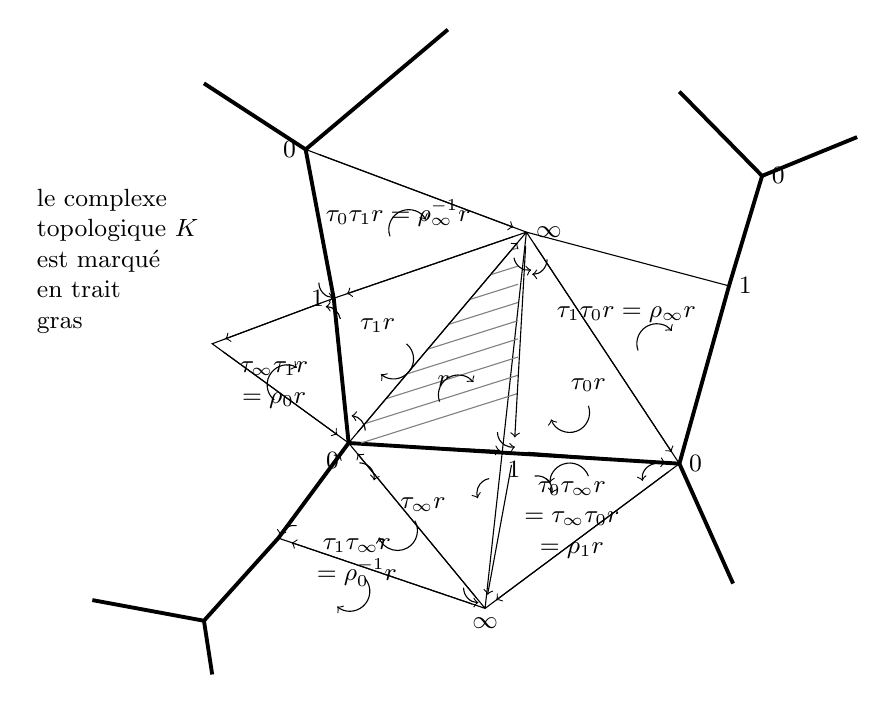
\begin{tikzpicture}[scale=1.05,every node/.style={font=\small}]
\coordinate (O) at (0,0);\coordinate (A) at (2,-.1);\coordinate (F) at (2.15,2.55);
\coordinate (B) at (-.18,1.75);\coordinate (U) at (-.52,3.55);\coordinate (R) at (4,-.25);
\coordinate (Q) at (4.6,1.9);\coordinate (V) at (5,3.23);\coordinate (D) at (1.65,-2);
\coordinate (L) at (-.85,-1.15);\coordinate (E) at (-1.65,1.2);
\draw[line width=1.4pt] (U)--(B)--(O)--(R)--(Q)--(V);
\draw[line width=1.4pt] (U)--(-1.75,4.35) (U)--(1.2,5) (V)--(4,4.25) (V)--(6.15,3.7) (R)--(4.65,-1.7);
\draw[line width=1.4pt] (O)--(L)--(-1.75,-2.15)--(-1.65,-2.8) (-1.75,-2.15)--(-3.1,-1.9);
\draw (U)--(F)--(B)--(E)--(O)--(F)--(R)--(D)--(O) (F)--(D) (L)--(D) (F)--(Q);
\begin{scope}\clip (O)--(F)--(A)--cycle;
\foreach \y in {0,.22,...,2.2}{\draw[gray,thin] (.15,\y)--(2.05,\y+.6);}\end{scope}
\foreach \p/\q in {U/F,F/B,B/E,E/O,O/F,F/R,R/D,D/O,D/L,L/O,F/A,A/D,O/A,A/R}{\draw[->,shorten >=5pt,shorten <=5pt] (\p)--(\q);}
\node[left] at (U) {$0$};\node[left] at (B) {$1$};\node[below left] at (O) {$0$};\node[right] at (F) {$\infty$};\node[right] at (Q) {$1$};\node[right] at (V) {$0$};\node[right] at (R) {$0$};\node[below] at (D) {$\infty$};
\node[below] at (A) {$1$};\node at (1.15,.75) {$r$};\node at (2.9,.7) {$\tau_0r$};\node at (.35,1.42) {$\tau_1r$};\node at (.9,-.75) {$\tau_\infty r$};
\node at (.6,2.78) {$\tau_0\tau_1r=\rho_\infty^{-1}r$};
\node at (3.36,1.55) {$\tau_1\tau_0r=\rho_\infty r$};
\node[align=center] at (-.9,.7) {$\tau_\infty\tau_1r$\\$=\rho_0r$};
\node[align=center] at (.1,-1.45) {$\tau_1\tau_\infty r$\\$=\rho_0^{-1}r$};
\node[align=center] at (2.7,-.93) {$\tau_0\tau_\infty r$\\$=\tau_\infty\tau_0r$\\$=\rho_1r$};
\foreach \x/\y/\aa/\bb in {1.1/.5/200/40,2.9/.45/20/-160,.7/1.2/50/-130,.8/-.94/30/-160,.5/2.5/200/30,3.5/1.12/200/40,-.9/.52/230/60,.2/-1.64/40/-130,2.9/-.4/20/180}{\draw[->] (\x,\y) arc (\aa:\bb:.24);}
\foreach \x/\y/\aa/\bb in {.2/.15/0/85,1.8/.13/180/280,2/2.24/190/280,2.4/2.22/0/-90,-.1/1.5/10/90,-.36/1.94/180/270,.13/-.24/90/-10,1.7/-.43/100/200,2.25/-.4/100/-10,3.7/-.25/100/190,-.63/-1/80/160,1.39/-1.75/180/270}{\draw[->] (\x,\y) arc (\aa:\bb:.18);}
\node[align=left,anchor=east] at (-1.7,2.2) {le complexe\\topologique $K$\\est marqué\\en trait\\gras};
\end{tikzpicture}}

\margin{\uline{NB} $\unsure{\sigma_i|\tau_i}$ change le sommet du type $i$ de $r$, en fixant les deux autres sommets}

Les opérations $\tau_0,\tau_1,\tau_\infty$ sont marquées sur la figure, ce sont les ``symétries'' p.r. aux côtés du triangle $r$ opposés aux sommets
\[
s=S_r^0,\quad\widetilde a=S_r^1,\quad\widetilde f=S_r^\infty
\]
de $r$ (sommets dits de type $0$ ou ``type-sommet'', type $1$ (ou ``type arête''), type $\infty$ (ou $2$) ou ``type-face''). On notera que les orientations induites par deux repères ``adjacents'' le long de l'arête commune sont les mêmes (ce qui s'explique par les \inserted{deux} orientations de la surface ambiante, au voisinage de cette arête, définies par $r$ et $r'$ respectivement, sont \uline{opposées}); elles sont données dans les sens $(0,1),(1,\infty),(\infty,0)$ sur les ``arêtes de types $\infty,0,1$'' respectivement. Par contre, les \deleted{orientations} \inserted{sens de rotation} autour des sommets communs de l'arête commune, définis par \deleted{\unsure{$r$ et $r'$}} respectivement par deux repères adjacents, sont \uline{opposées}. La figure montre en tout neuf repères, savoir $r$ et ceux qui s'en déduisent en appliquant \deleted{\unsure{de}} les opérations $\tau_i$ ($i\in\{0,1,\infty\}$), et en \deleted{\unsure{les réitérant}} \inserted{recommençant} une fois
\diagram{$\left\{\begin{array}{llll}
r&\tau_0r,\tau_1r,\tau_\infty r&\tau_1\tau_0r=\rho_\infty r,&\tau_0\tau_1r=\rho_\infty^{-1}r\\
&&\multicolumn{2}{l}{\tau_0\tau_\infty r=\rho_1r\unsure{\ne|=}\tau_\infty\tau_0r=\rho_1^{-1}r}\\
&&\multicolumn{2}{l}{\tau_\infty\tau_1r=\deleted{\unsure{\rho_\infty}}\rho_0r,=\tau_\infty\tau_0r=\rho_0^{-1}r}
\end{array}\right.$}
(il y aurait 10 repères, au lieu de $9=1+3+(2+1+2)$, s'il n'y avait \unsure{ici} la relation
\[
\tau_0\tau_\infty=\tau_\infty\tau_0\qquad\text{i.e.}\quad\rho_1=\rho_1^{-1}\qquad\text{i.e.}\quad\rho_1^2=1
\]
\mspage{54}

\scanpage{56}
\mspage{3}

où maintenant ``spéciaux'' signifie que $\rho_1=\tau_0\tau_\infty$ opère sans points fixes.

Si on a une carte orientée, sa \deleted{\unsure{considérer}} carte duale munie de la \uline{même orientation de la surface sous-jacente commune}, est appelée la \uline{carte orientée duale}. On aura alors
\[
(9)\qquad R^+(\check C)=R^-(C),\quad R^-(\check C)=R^+(C)
\]
i.e. les repères directs pour l'une des deux cartes en dualité sont ceux qui sont inverses pour l'autre.

On se libère de la condition de restriction aux $G_2^\circ$-ensembles finis \uline{spéciaux}, en introduisant une notion un peu plus générale de carte cellulaire, en \deleted{\unsure{admettant des}} \inserted{introduisant la notion} d'\uline{arête pliée} -- Techniquement, on a, en plus de $K$, une partie finie $S\subset K$, \inserted{(ens. des sommets)} \unsure{qui contient} tous les sommets topologiques, sauf éventuellement certains sommets d'ordre 1 ou points-bouts de $K$.

\figure{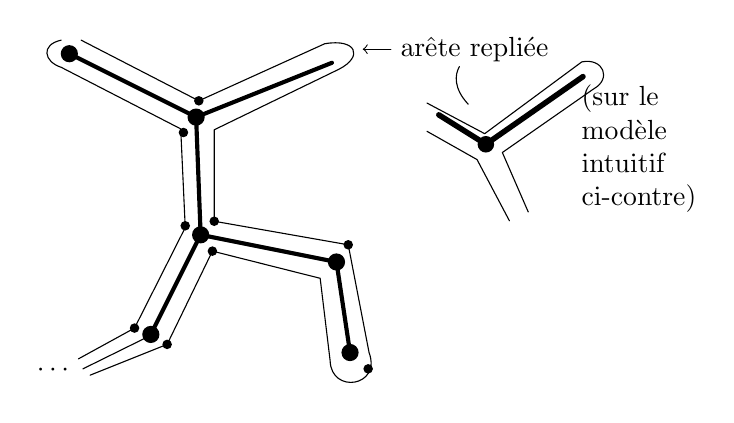
\begin{tikzpicture}[scale=1.15,line cap=round,line join=round]
\draw[line width=1.5pt] (-1.4,2.6)--(0,1.9)--(1.5,2.5) (0,1.9)--(.05,.6)--(-.5,-.5) (.05,.6)--(1.55,.3)--(1.7,-.7);
\draw (-1.49,2.75) .. controls (-1.72,2.7) and (-1.68,2.51) .. (-1.49,2.45)--(-.17,1.77)--(-.12,.68)--(-.68,-.43)--(-1.3,-.77);
\draw (-1.27,2.75)--(.03,2.08)--(1.42,2.71) .. controls (1.77,2.77) and (1.85,2.57) .. (1.58,2.43)--(.2,1.76)--(.2,.75)--(1.68,.49)--(1.91,-.7) .. controls (2.05,-1.08) and (1.49,-1.16) .. (1.48,-.79)--(1.37,.12)--(.18,.42)--(-.32,-.61)--(-1.17,-.95);
\draw (-1.25,-.88)--(-.52,-.52);
\foreach \x/\y in {-1.4/2.6,0/1.9,.05/.6,-.5/-.5,1.55/.3,1.7/-.7}{\fill (\x,\y) circle (2.7pt);}
\foreach \x/\y in {-.14/1.73,.03/2.08,-.12/.7,.2/.75,.18/.42,-.68/-.43,-.32/-.61,1.68/.49,1.9/-.88}{\fill (\x,\y) circle (1.5pt);}
\node at (-1.58,-.9) {$\cdots$};
\draw[<-] (1.84,2.65)--(2.15,2.65);\node[anchor=west] at (2.15,2.65) {arête repliée};
\begin{scope}[shift={(3.2,1.6)},scale=.65]
\draw[line width=2pt] (-.8,.5)--(0,0)--(1.65,1.15);
\fill (0,0) circle (4pt);
\draw (-1,.7)--(-.02,.18)--(1.63,1.4) .. controls (2,1.47) and (2.14,1.11) .. (1.83,.94)--(.28,-.14)--(.72,-1.15);
\draw (-1,.22)--(-.15,-.26)--(.4,-1.3);
\draw (-.3,.68) .. controls (-.55,.95) and (-.53,1.18) .. (-.45,1.32);
\end{scope}
\node[align=left,anchor=west] at (4.15,1.55) {(sur le\\modèle\\intuitif\\ci-contre)};
\end{tikzpicture}}
\margin{les sommets marqués sont marqués en gros, le contour de la découpe $D(X/K)$ en trait fin, les sommets sur le bord de la découpe sont \deleted{\unsure{tous}} figurés aussi.}

On reformule directement les axiomes en termes de $S\subset K\subset X$. Du point de vue des repères le long d'une arête pliée il y a deux repères (au lieu de quatre comme dans le cas précédemment étudié)

\mspage{55}

\scanpage{57}
\figure{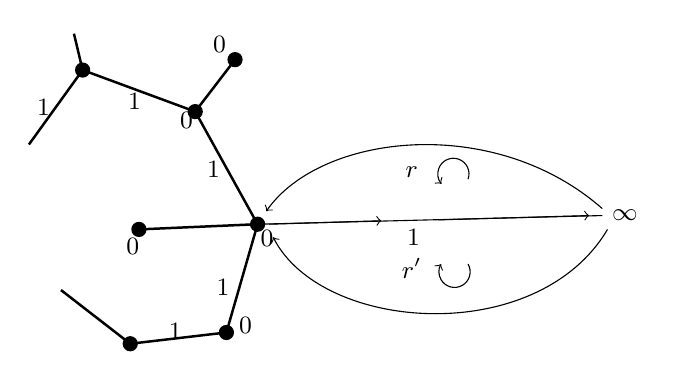
\begin{tikzpicture}[scale=1.1,every node/.style={font=\small}]
\draw[line width=.9pt] (-1.5,3.4)--(-1.4,2.98)--(-.1,2.5)--(.62,1.2)--(.26,-.05)--(-.85,-.18)--(-1.65,.44);
\draw[line width=.9pt] (-1.4,2.98)--(-2.02,2.12) (-.1,2.5)--(.36,3.1) (.62,1.2)--(-.75,1.14);
\draw (.62,1.2)--(4.6,1.3);
\draw[->] (.75,1.2)--(2.05,1.24);\draw[->] (2.7,1.25)--(4.45,1.3);
\draw[->] (4.6,1.38) .. controls (3.35,2.48) and (1.35,2.25) .. (.72,1.35);
\draw[->] (4.66,1.14) .. controls (3.85,-.23) and (1.36,-.05) .. (.8,1.05);
\node at (2.4,1.8) {$r$};\node at (2.4,.69) {$r'$};
\draw[->] (3.05,1.72) arc (-20:220:.18);\draw[->] (3.05,.74) arc (30:-210:.18);
\foreach \x/\y in {-1.4/2.98,-.1/2.5,.36/3.1,.62/1.2,-.75/1.14,.26/-.05,-.85/-.18}{\fill (\x,\y) circle(2.5pt);}
\foreach \x/\y in {-.2/2.4,.18/3.27,.73/1.04,-.82/.94,.48/.03}{\node at (\x,\y) {$0$};}
\foreach \x/\y in {-1.85/2.55,-.8/2.62,.11/1.83,.22/.47,-.33/-.04,2.42/1.05}{\node at (\x,\y) {$1$};}
\node[right] at (4.6,1.3) {$\infty$};
\end{tikzpicture}}
\[
(10)\quad\left\{\begin{aligned}
r'&=\tau_\infty r=\tau_0r\deleted{\unsure{r}}\\
\text{i.e.}\quad\tau_0\tau_\infty r&=r\quad\text{i.e.}\quad\rho_1r=r
\end{aligned}\right.
\]
\deleted{\figure{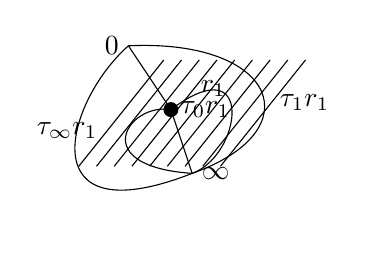
\begin{tikzpicture}[scale=.9]
\draw (0,1.8)--(.6,.9)--(.9,0);
\fill (.6,.9) circle(3pt);
\draw (0,1.8) .. controls (2.1,1.9) and (2.6,.6) .. (.9,0) .. controls (-1.4,-.9) and (-.9,1) .. (0,1.8);
\draw (.6,.9) .. controls (1.8,1.8) and (1.6,.25) .. (.9,0) .. controls (-.6,.1) and (0,1) .. (.6,.9);
\node[left] at (0,1.8) {$0$};\node[right] at (.9,0) {$\infty$};
\node at (1.2,1.2) {$r_1$};\node[left] at (-.3,.6) {$\tau_\infty r_1$};\node[right] at (.6,.9) {$\unsure{\tau_0r_1}$};\node[right] at (2,1) {$\unsure{\tau_1r_1}$};
\foreach \x in {-.7,-.45,...,1.3}{\draw (\x,.1)--(\x+1.2,1.6);}
\end{tikzpicture}}}

Les arêtes \unsure{aplaties} correspondent 1-1 aux ``sommets de type 1'' (de la subdivision barycentrique) qui sont des sommets topologiques (néc\textsuperscript{t}. d'ordre 1) de $K$. Et elles correspondent 1-1 aux points fixes de $\rho_1=\unsure{\sigma_0\sigma_\infty|\tau_0\tau_\infty}$ opérant sur $R$.

Pour un pt. bout de $K$ qui est un sommet marqué de $K$ (i.e. un sommet de type 1 de la subdivision barycentrique) on a la situation ci-contre
\figure{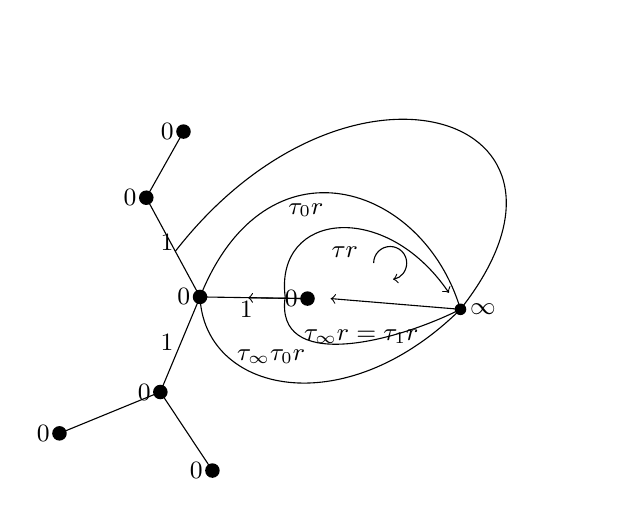
\begin{tikzpicture}[scale=1.05,every node/.style={font=\small}]
\draw (-.2,2.5)--(-.65,1.7)--(0,.5)--(-.48,-.65)--(-1.7,-1.15) (-.48,-.65)--(.15,-1.6) (0,.5)--(1.3,.48);
\foreach \x/\y in {-.2/2.5,-.65/1.7,0/.5,-.48/-.65,-1.7/-1.15,.15/-1.6,1.3/.48}{\fill (\x,\y) circle(2.5pt);\node[left] at (\x,\y) {$0$};}
\foreach \x/\y in {-.4/1.16,-.4/-.05,.56/.35}{\node at (\x,\y) {$1$};}
\draw (-.3,1.05) .. controls (1.8,3.75) and (5,2.7) .. (3.15,.35);
\draw (0,.5) .. controls (.8,2.5) and (2.7,1.87) .. (3.15,.35) .. controls (1.73,-1.05) and (.05,-.65) .. (0,.5);
\draw[->] (3.15,.35)--(1.58,.48);
\draw[->] (1.26,.48)--(.58,.49);
\draw[->] (1.03,.5) .. controls (.9,1.53) and (2.24,1.68) .. (3.01,.55);
\draw (1.03,.5) .. controls (.9,-.4) and (2.31,-.07) .. (3.15,.35);
\fill (3.15,.35) circle(2pt);\node[right] at (3.15,.35) {$\infty$};
\node at (1.28,1.55) {$\tau_0r$};\node at (1.75,1.04) {$\deleted{\unsure{\tau}}r$};
\draw[->] (2.1,.91) arc (180:-80:.2);
\node at (.86,-.22) {$\tau_\infty\tau_0r$};\node at (1.95,.02) {$\unsure{\tau_\infty r=\tau_1r}$};
\end{tikzpicture}}
, il y a bien \uline{4} repères distincts adjacents à l'arête qui aboutit en ce sommet -- si on prend l'un des deux qui \deleted{\unsure{ont pour}} \inserted{ont comme} \deleted{``plié''} \inserted{``pli''} le \deleted{sommet} envisagé, on aura
\[
(11)\qquad\tau_1r=\tau_\infty r\qquad\text{i.e.}\quad\rho_0r=r
\]
ce qui caractérise les sommets envisagés (ils sont en corr. biunivoque avec les paires de repères $\{r,r'\}$ telles que $r'=\tau_1r=\tau_\infty r$, d'où $r=\tau_1r'=\tau_\infty r'$).

\deleted{\unsure{La condition}} La condition (11) n'\unsure{empêche} pas qu'on

\mspage{56}

\scanpage{58}
\mspage{4}

puisse avoir \deleted{\unsure{aussi}} même
\[
\tau_1r=\tau_\infty r=\tau_0r
\]
i.e. qu'on soit dans le cas (10) (purement comb.: gr. d'op. $G_2$, avec les $\unsure{\sigma_i|\tau_i}$ opérant sans pts fixes) cela signifie que le point de \uline{type 1} du repère envisagé est un pli (les points de type 0 ne peuvent l'être, par définition).

Grâce à l'introduction des arêtes pliées, dans la équiv. de catégories (8), il n'est plus néc. d'introduire l'hyp que $\rho_1$ opère sans pt fixe -- et dans l'équivalence (1), il n'y a plus lieu de supposer que $\rho_1$ (alias $\sigma$) opère ss pt fixes -- par contre la condition que les $\unsure{\sigma_i|\tau_i}$ opèrent sans points fixes demeure provisoirement (mais il serait facile maintenant de s'en affranchir \deleted{\unsure{?}} cf plus bas\ldots)).

\textcircled{2} On a dans ces considérations un rôle particulier pour l'indice $1\in\{0,1,\infty\}$, du fait que l'on a
\[
\rho_1^2=1,
\]
on peut s'en défaire, en réintroduisant
\[
(12)\qquad\Pi_{03}^{\deleted{\unsure{\omega}}\tau}=\{\tau_0,\tau_1,\tau_\infty\mid\tau_0^2=\tau_1^2=\tau_\infty^2=1\}
\]
(sans condition $(\tau_0\tau_\infty)^2=1$ !), et le sous-groupe d'indice 2
\margin{$\Pi_{03}$ \unsure{est le noyau de} \deleted{$\unsure{\Pi_{03}}$}
\diagram{\begin{tikzcd}[column sep=small,row sep=small]
\Pi_{03}^{\tau}\arrow[r]&\mathbb Z/2\\
\unsure{\sigma_i|\tau_i}\arrow[r,mapsto]&1\bmod2
\end{tikzcd}}}
\[
(13)\qquad\Pi_{03}=\{\rho_0,\rho_1,\rho_\infty\mid\rho_\infty\rho_1\rho_0=1\}
\]
\mspage{57}

\scanpage{59}
en prenant encore, comme dans 5
\[
(14)\qquad\rho_\infty=\tau_1\tau_0,\quad\rho_1=\tau_0\tau_\infty,\quad\rho_0=\tau_\infty\tau_1.
\]
On a donc
\[
(15)\qquad G_2\simeq\unsure{\Pi_{03}^\tau|\widetilde\Pi_{03}^\tau}/\langle\rho_1^2\rangle,
\quad G_2^\circ\simeq\Pi_{03}/\langle\rho_1^2\rangle
\]
\deleted{Cette fois} \inserted{Ici} \deleted{\unsure{G}} $\Pi_{03}^\tau$ apparaît comme le groupe ``classifiant'' pour la structure de ``\uline{carte tri-angulaire pondérée}'' (par $\{0,1,\infty\}$), i.e. une carte $C=(X,K)$ au sens de \unsure{p.g 1}, avec \deleted{l'ensemble} une application
\diagram{\begin{tikzcd}[column sep=large]
(16)\quad\begin{array}{c}S\\[-.2em]\text{ens des}\\\text{sommets}\\\text{(ordinaires)}\\\text{de la carte (\uline{pas} d'une}\\\text{subd. barycentrique!)}\end{array}\arrow[r]&\{0,1,\infty\}
\end{tikzcd}}
ayant la propriété que pour toute face $f$, l'application (16) induit une bijection de l'ens des sommets de $f$ avec $\{0,1,\infty\}$. L'ensemble des \uline{repères} (au sens de la théorie \inserted{tri-angulaire} pondérée, en cas de possibilité de confusion on dira ``repères pondérés'') de $X$ est par définition l'ens de ses faces, et $\unsure{\sigma_i|\tau_i}$ ($i\in\{0,1,\infty\}$) est le \deleted{\unsure{symé}} repère symétrique p.r. au \deleted{\unsure{repère le}} côté du repère opposé au \deleted{le} sommet de type $i$. L'\uline{ordre} des \uline{sommets} est pair on appelle \uline{ordre réduit} d'un sommet le quotient de l'ordre par \deleted{\unsure{2}} deux.

\mspage{58}

\scanpage{60}
\mspage{5}

\figure{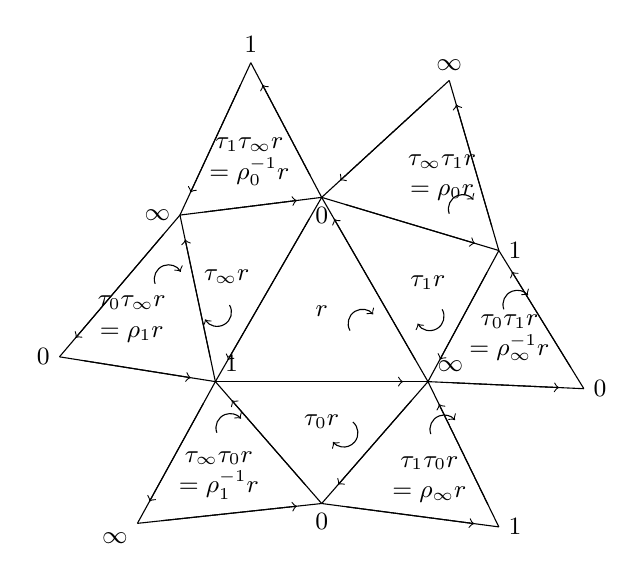
\begin{tikzpicture}[scale=.9,every node/.style={font=\small}]
\coordinate (T) at (0,2.6);\coordinate (L) at (-1.5,0);\coordinate (R) at (1.5,0);
\coordinate (OL) at (-2,2.35);\coordinate (TL) at (-1,4.5);\coordinate (TR) at (1.8,4.25);
\coordinate (OR) at (2.5,1.85);\coordinate (FR) at (3.7,-.1);\coordinate (BR) at (2.5,-2.05);
\coordinate (B) at (0,-1.72);\coordinate (BL) at (-2.6,-2);\coordinate (FL) at (-3.7,.35);
\foreach \p/\q in {T/L,L/R,R/T,T/TL,TL/OL,OL/T,T/OR,OR/TR,TR/T,FL/L,L/OL,OL/FL,FR/OR,OR/R,R/FR,B/L,L/BL,BL/B,B/BR,BR/R,R/B}{\draw (\p)--(\q);\draw[->,shorten >=9pt,shorten <=9pt] (\p)--(\q);}
\node[below] at (T) {$0$};\node[above right] at (L) {$1$};\node[above right] at (R) {$\infty$};
\node[left] at (OL) {$\infty$};\node[above] at (TL) {$1$};\node[above] at (TR) {$\infty$};\node[right] at (OR) {$1$};
\node[right] at (FR) {$0$};\node[right] at (BR) {$1$};\node[below] at (B) {$0$};\node[below left] at (BL) {$\infty$};\node[left] at (FL) {$0$};
\node at (0,1) {$r$};\node at (-1.34,1.48) {$\tau_\infty r$};\node at (1.5,1.4) {$\tau_1r$};\node at (0,-.57) {$\tau_0r$};
\node[align=center] at (-1.02,3.1) {$\tau_1\tau_\infty r$\\$=\rho_0^{-1}r$};
\node[align=center] at (1.7,2.88) {$\tau_\infty\tau_1r$\\$=\rho_0r$};
\node[align=center] at (-2.68,.88) {$\tau_0\tau_\infty r$\\$=\rho_1r$};
\node[align=center] at (2.65,.62) {$\tau_0\tau_1r$\\$=\rho_\infty^{-1}r$};
\node[align=center] at (-1.45,-1.32) {$\tau_\infty\tau_0r$\\$=\rho_1^{-1}r$};
\node[align=center] at (1.52,-1.38) {$\tau_1\tau_0r$\\$=\rho_\infty r$};
\foreach \x/\y/\aa/\bb in {.4/.72/210/40,-1.3/1.08/30/-150,1.7/1.02/30/-150,.44/-.57/50/-140,-2.35/1.38/200/30,2.57/1.02/200/40,1.8/2.37/200/40,-1.48/-.72/200/40,1.54/-.74/200/40}{\draw[->] (\x,\y) arc (\aa:\bb:.2);}
\end{tikzpicture}}

Les propriétés d'orientation de la figure sont les mêmes que celles expliquées p. $2'$, la figure est plus jolie car de nature plus symétrique. \unsure{Du reste}, dans des cas particuliers certains des 10 \deleted{\unsure{triangles}} \inserted{triangles} repères de la figure peuvent coïncider (ex: octaèdre, ou exemple plus dégénéré encore, le cas ``orienté universel''
\figure{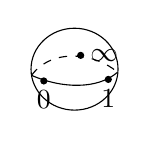
\begin{tikzpicture}[scale=.65]
\draw (0,0) ellipse (.85 and .8);
\draw (-.84,-.12) .. controls (-.25,-.38) and (.45,-.4) .. (.84,-.06);
\draw[dashed] (-.84,-.12) .. controls (-.42,.44) and (.43,.3) .. (.84,-.06);
\fill (-.6,-.23) circle(2pt);\fill (.66,-.2) circle(2pt);\fill (.12,.27) circle(2pt);
\node[below] at (-.6,-.23) {$0$};\node[below] at (.66,-.2) {$1$};\node[right] at (.12,.27) {$\infty$};
\end{tikzpicture}}.

Ici l'équivalence de catégories ad hoc
\diagram{\begin{tikzcd}[column sep=large]
(17)\quad\begin{array}{c}\text{cartes isot. tri-angulaires}\\\text{pondérées}\end{array}\arrow[r,"\approx"]&\begin{array}{c}\Pi_{03}^\tau\text{-ensembles}\\\text{finis spéciaux}\end{array}
\end{tikzcd}}
est en termes des ens finis $R$ à opérateurs involutifs $\tau_i$ ($i\in\{0,1,\infty\}$) \uline{sans points fixes}, sans plus.

Définissant les cartes tri-angulaires pondérées orientées comme dans le cas des cartes ordinaires, par une orientation de la surface top. sous-jacente, on voit que cette notion se définit encore combinatoirement par la donnée d'un sous-ens. $R^+(X)$ de l'ens $R(X)$ des repères pondérés de $X$, satisfaisant (6 bis), i.e. (7), \deleted{bis.}\inserted{(7 bis)} \deleted{\unsure{et}} on a encore posé
\[
R^-(X)=R(X)\setminus R^+(X).
\]
On a alors

\mspage{59}

\scanpage{61}
\diagram{\begin{tikzcd}[column sep=large]
(18)\quad\text{Cartes (isotop) tri-angulaires pondérées orientées}\arrow[r,"\approx"]&(\Pi_{03}\text{-Ens})\\
X\arrow[r,mapsto]&R^+(X)
\end{tikzcd}}

\margin{\uline{NB} Il n'y a pas d'autre condition sur l'ens $R$ \unsure{ayant} $\Pi_{03}$ comme groupe d'opérateurs que d'être fini\ldots}

La notion de ``carte duale'' se remplace ici par la notion de transformation d'une carte par une ``ré-indexation'' des sommets, via un
\[
g\in\mathfrak S_3\overset{\mathrm{déf}}=\mathfrak S_{\{0,1,\infty\}}.
\]
Je n'insiste pas sur ces développements, essentiellement triviaux, sauf pour noter la formule
\[
(18)\qquad R^+(X^g)=R^{\operatorname{sg}g}(X)
\qquad\begin{array}{l}g\in\mathfrak S_3\\\operatorname{sg}g\text{ la signature}\\\text{de }g\end{array}
\]

\textcircled{3} Par les considérations précédentes, et notamment par les isom (15)
\[
\begin{split}
G_2&\simeq\Pi_{03}^{\tau}/\langle\rho_1^2\rangle\\
G_2^+&\simeq\Pi_{03}/\langle\rho_1^2\rangle,
\end{split}
\]
la cat. \inserted{isotopique} des cartes finies (avec arêtes pliées) apparaît comme équivalente à une sous-catégorie pleine de la catégorie \inserted{isotop} des cartes finies tri-angulaires pondérées, et idem pour la version orientée. D'autre part, on a
\[
(19)\qquad\Pi_{03}\simeq\Pi_1(U_{03},\unsure{P_+^*|P_*^+})
\]
où \unsure{$U_{03}$:}
\[
(20)\qquad U_{03}=\mathbf P^1(\mathbf C)\setminus\{0,1,\infty\}
\]
\deleted{$P_*$ étant} $P_*$ étant un pt \deleted{quel} de l'hémisphère supérieur -- il est commode de prendre
\[
P_*=-\overline\zeta,\qquad\zeta=\exp 2i\pi/3.
\]

\mspage{60}
